\chapter{Results}\label{sec:results}

The following presents the results from different experiments on the dummy and real-world BSD datasets. All defined research questions in chapter \ref{chapter:research_approach} were investigated on the dummy dataset. The results are presented in section \ref{sec:results_dummy_dataset}. Excluding the labeled MMD-loss evaluation, these research questions were also analyzed on the real-world BSD dataset. The outcomes are discussed in section \ref{sec:results_real_world_dataset}. The overall PHM performance of the proposed model is presented in chapter \ref{ch:PHM_performance}. In the last chapter \ref{sec:Performance_overview}, the experimental findings from both datasets are concluded.




\section{Dummy Dataset}\label{sec:results_dummy_dataset}
Several experiments were performed on the dummy dataset to analyze the effects of the MMD-loss in a simplified setting and to make initial estimates about its applicability for PHM tasks. The model architecture used in these experiments was the same as described in section \ref{sec:model}. In sections \ref{sec:Balancing Cross-Entropy and MMD loss} and \ref{sec:Differences of labeled and unlabeled MMD loss}, the influence of the GAMMA choice and the differences between the labeled and unlabeled MMD-loss were analyzed. In the experiments executed in this context, a single SGD optimizer with a learning rate of 0.01 was used. All layers were trained simultaneously with a weighted average of an MMD- and a source CE-loss. The visualization of the MMD-loss influence on the latent feature space representations became more visible when using that simplified model optimization. Chapter \ref{cnn_mmd_dummy} evaluates the application of MMD-losses in different latent feature spaces. In the corresponding experiments the models were optimized as explained in section \ref{sec:Proposed_training}. The MMD-losses were evaluated according to the performance of the models trained with them. In order to evaluate the MMD-losses for the real application, the more sophisticated model training, which was also applied to the real-world BSD dataset, was used.


\subsection{Influence of the GAMMA Choice on the Domain Adaptation Performance} \label{sec:Balancing Cross-Entropy and MMD loss}

The following section evaluates the influence of the hyperparameter GAMMA on the training. The FC2 latent feature representations of the source and target domain samples during different epochs are visualized in figure \ref{fig:point_cloud_mmd}. The corresponding MMD-loss and source CE-loss development are shown in figure \ref{fig:learning_curves_influence_mmd_feature_extractor}.
\begin{itemize}
    \item [\textbf{Small GAMMA}]:
    When a very small GAMMA was selected, the source CE-loss was reduced, whereas the MMD-loss was increased throughout the training (see figure \ref{fig:learning_curves_influence_mmd_feature_extractor}). This showed the dominance of the source CE-loss. Instead of reducing the domain discrepancy, the model training focused on predicting the source samples correctly. The model's performance was solely improved on the source domain but the knowledge was not properly transferred to the target domain. Since the influence of the MMD-loss was negligible, the domain discrepancy was not reduced properly. Therefore, the separability and compactness of the classes were low and the class representations did not overlap properly across the domains (see figure \ref{fig:point_cloud_mmd}).
    \item [\textbf{Medium GAMMA}]:
    When the GAMMA was chosen correctly, the source CE- and MMD-loss were reduced simultaneously (see figure \ref{fig:learning_curves_influence_mmd_feature_extractor}). For this GAMMA choice, the model was optimized to correctly classify the source domain samples, while reducing the domain discrepancy. Knowledge learned from the source domain was successfully transferred to the target domain. In this case, the training profited from both losses equally. An optimization with multiple goals was achieved and neither of them solely dominated the training. Compared to the smaller GAMMA choice, the class distributions in the latent feature space showed increased compactness and separability of the classes in both domains (see figure \ref{fig:point_cloud_mmd}). Especially for class 1, the point clouds were denser and there were fewer outliers far away from their corresponding class center (see figure \ref{fig:point_cloud_mmd}). The distance between different classes was increased and the subspace separating those was less dense (see figure \ref{fig:point_cloud_mmd}). The point clouds of equal classes and different domains were structured more similarly and their overlap was improved (see figure \ref{fig:point_cloud_mmd}). This showed that the samples were successfully transferred in a more domain-invariant feature space, where the domain discrepancy was reduced.
    \item [\textbf{Large GAMMA}]:
    When a very large GAMMA was selected, the MMD-loss was reduced efficiently, whereas the source CE-loss was increased throughout the training (see figure \ref{fig:learning_curves_influence_mmd_feature_extractor}). The correct prediction of source domain samples became irrelevant. Since the target labels were unknown, the MMD-loss was calculated between the source and target domain samples of the same and different classes. Therefore, the MMD-loss reduced the inter- and intra-class distance between the latent feature representations of the source and target domain. The compactness of the classes was increased but their separability was reduced. This led to a trivial solution, where all latent feature representations collapsed to a point- or needle-like subspace (see \ref{fig:point_cloud_mmd}). The classification task became more challenging for that specific latent feature representation.
\end{itemize}

\begin{figure}[H]
  \centering
  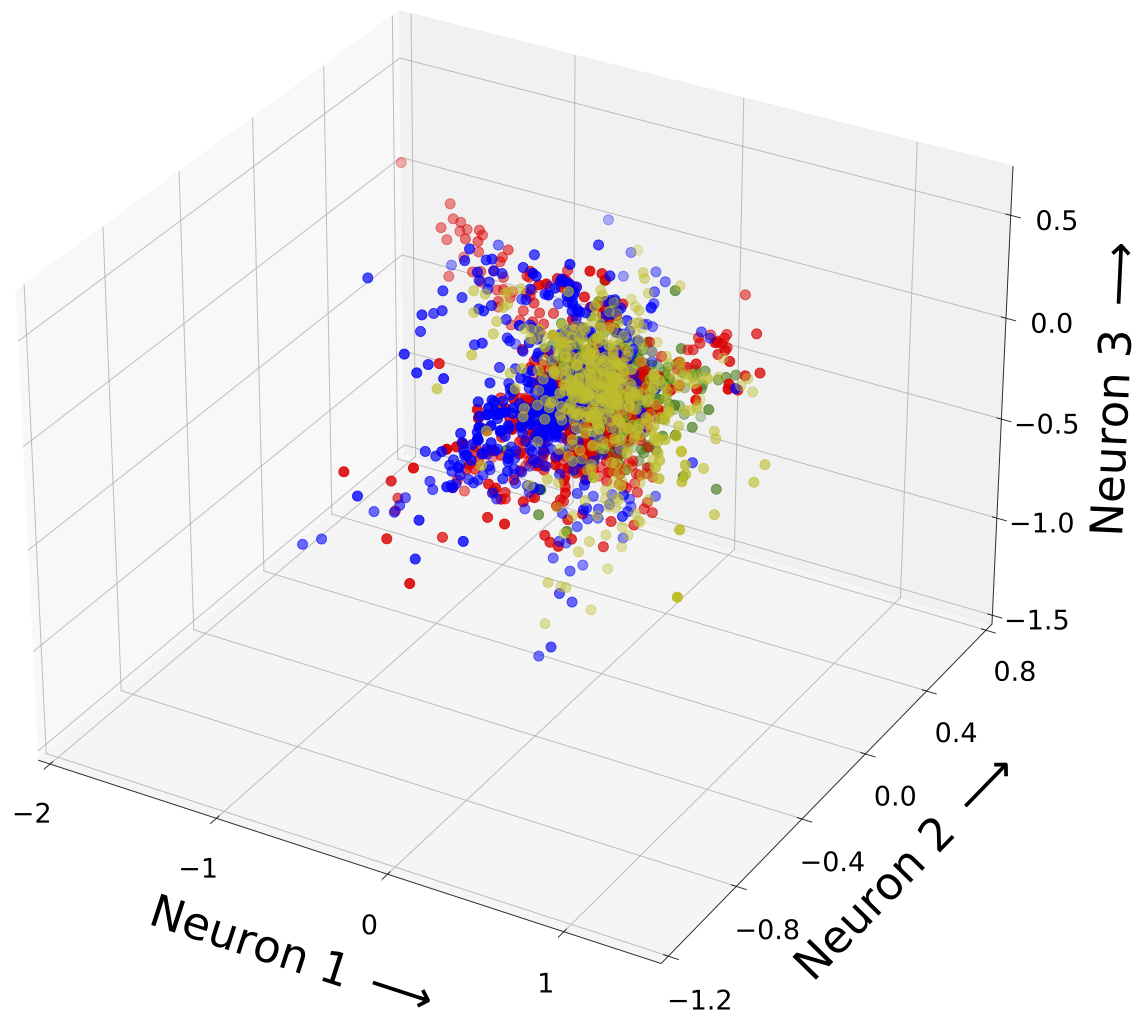
\includegraphics[width=.48\textwidth]{GAMMA_Influence_dummy_distribution/Dummy_distribution_0_GAMMA_0_001.png}
  \hspace{.4cm}
  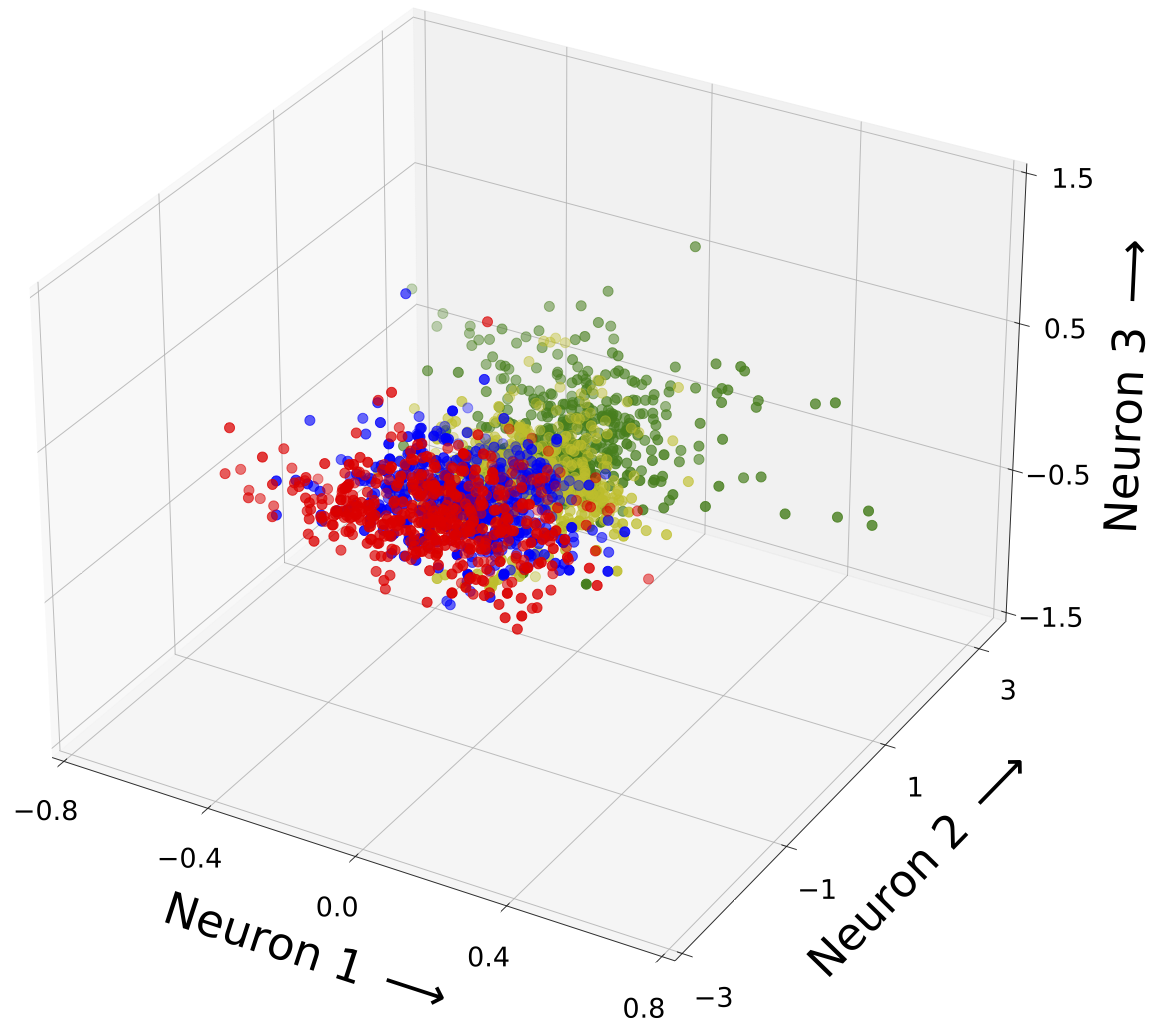
\includegraphics[width=.48\textwidth]{GAMMA_Influence_dummy_distribution/Dummy_distribution_8_GAMMA_0_001.png}

  \vspace{.1cm}

  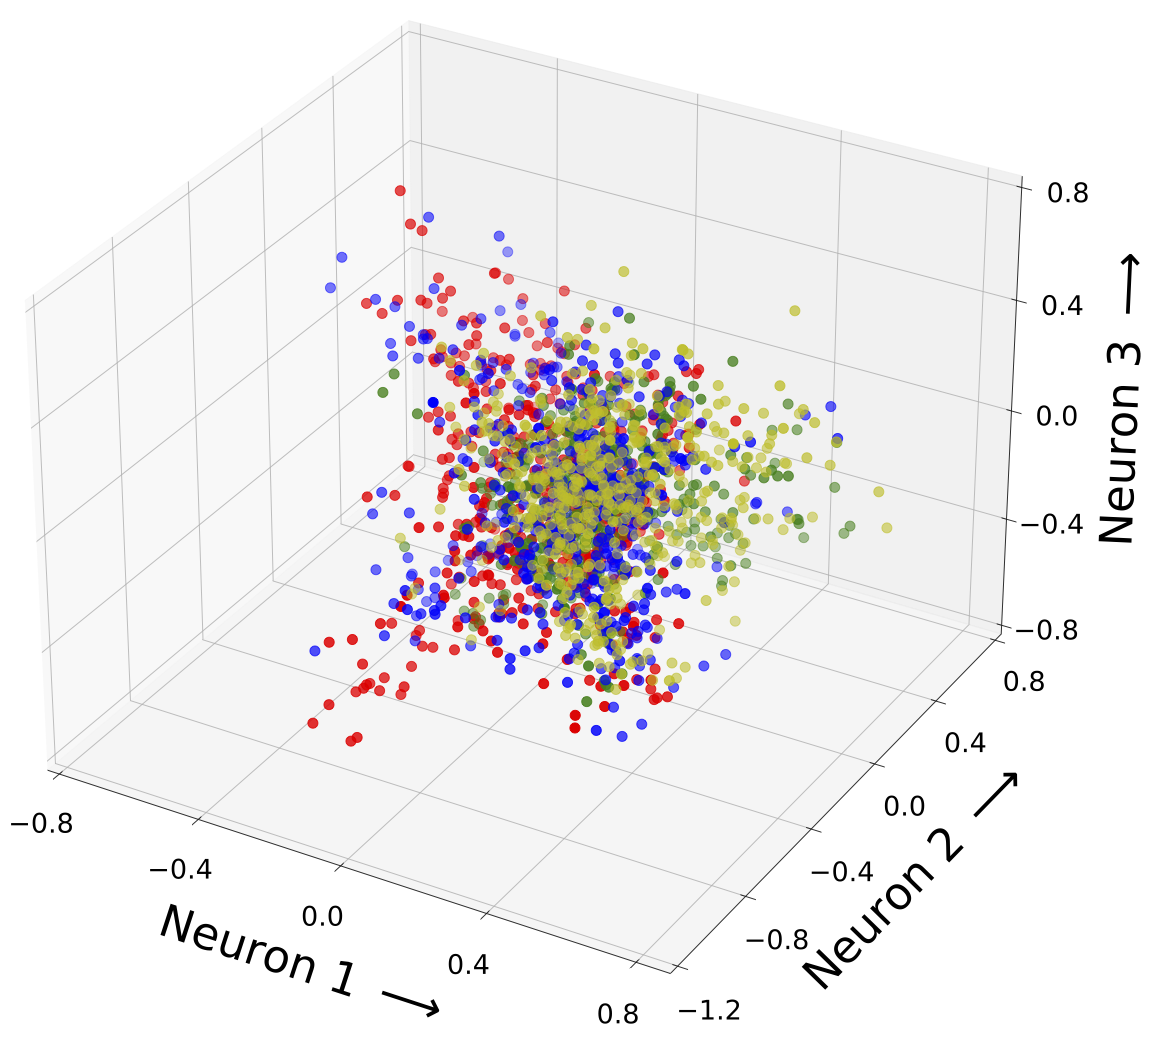
\includegraphics[width=.48\textwidth]{GAMMA_Influence_dummy_distribution/Dummy_distribution_0_GAMMA_0_1.png}
  \hspace{.4cm}
  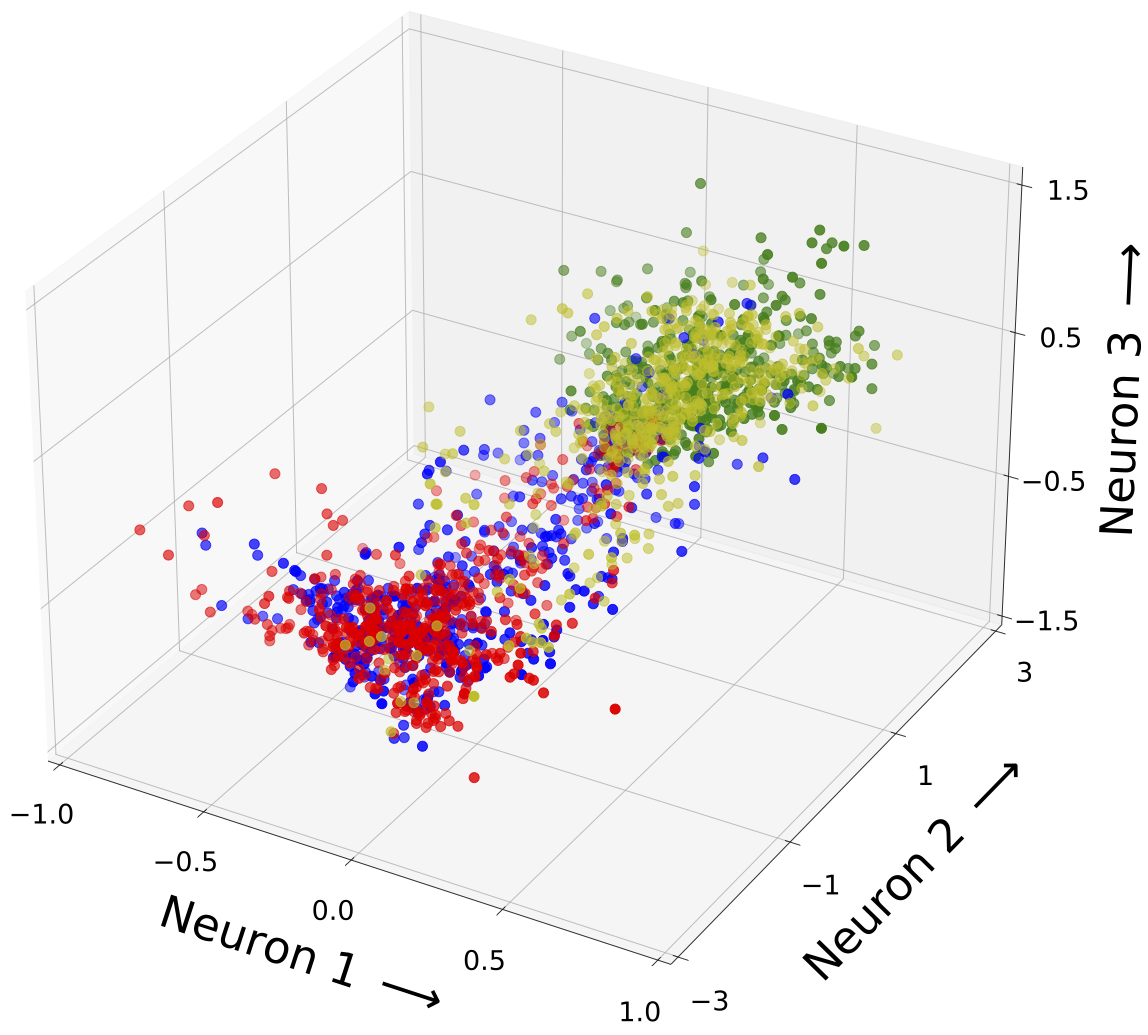
\includegraphics[width=.48\textwidth]{GAMMA_Influence_dummy_distribution/Dummy_distribution_8_GAMMA_0_1.png}

  \vspace{.1cm}

  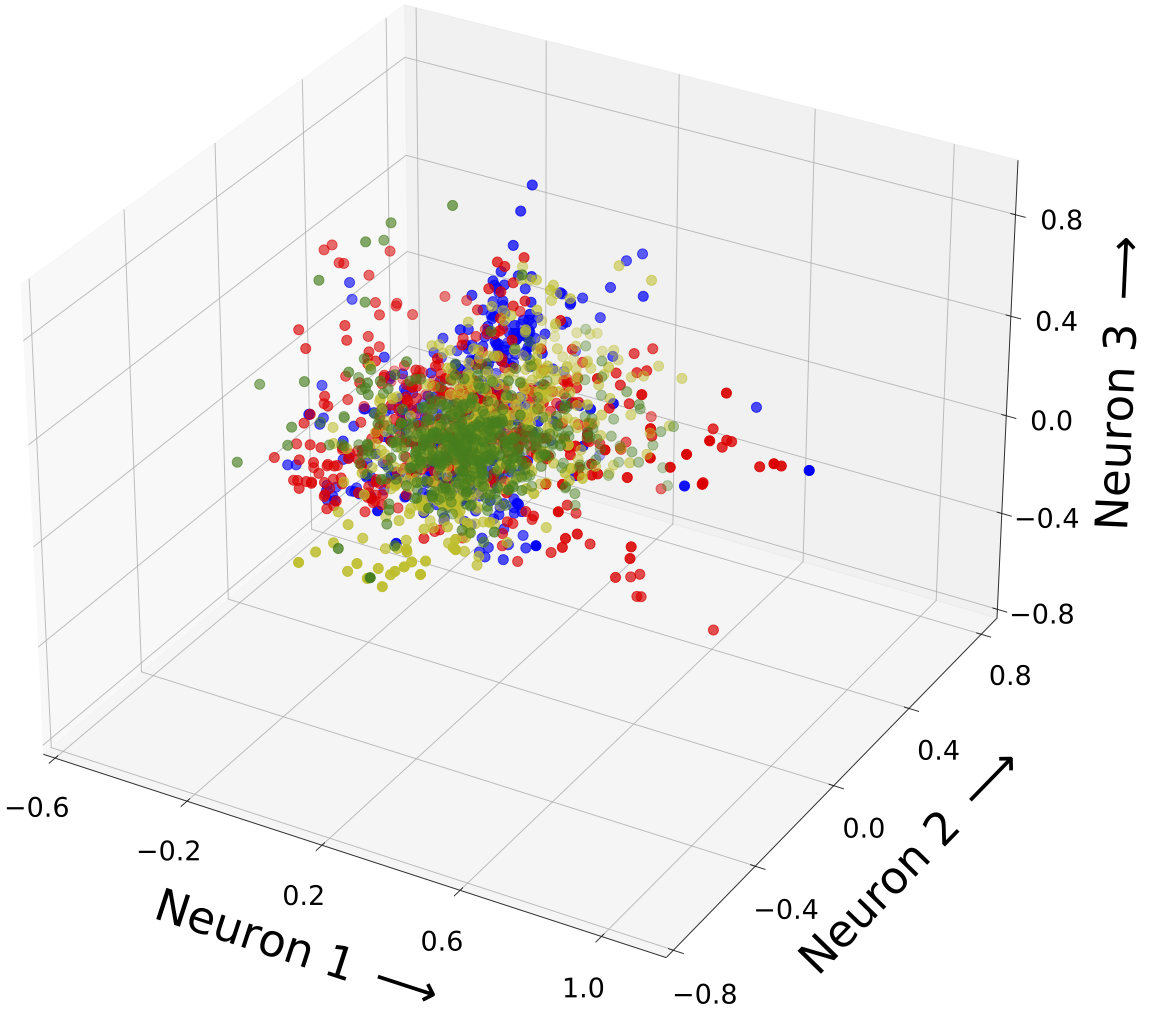
\includegraphics[width=.48\textwidth]{GAMMA_Influence_dummy_distribution/Dummy_distribution_0_GAMMA_20.png}
  \hspace{.4cm}
  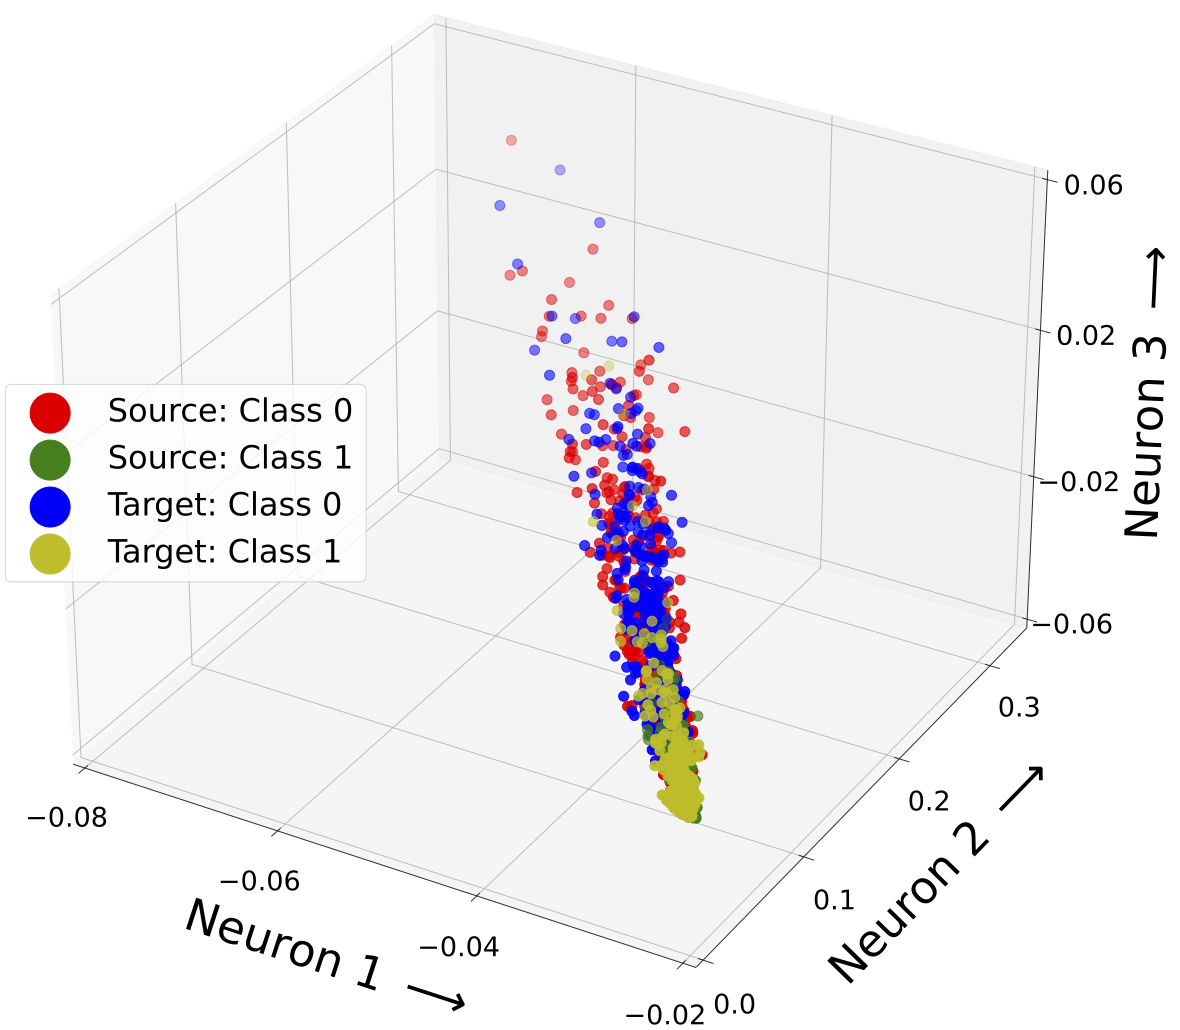
\includegraphics[width=.48\textwidth]{GAMMA_Influence_dummy_distribution/Dummy_distribution_8_GAMMA_20.png}
 

  \caption{Data distribution: Influence of the GAMMA choice on the model training, GAMMA = 0.05 (top), GAMMA = 0,4 (middle), GAMMA = 20 (bottom), Epoch = 0 (left) , Epoch = 8 (right)}
  \label{fig:point_cloud_mmd}
\end{figure}


\begin{figure}[H]
  \centering
  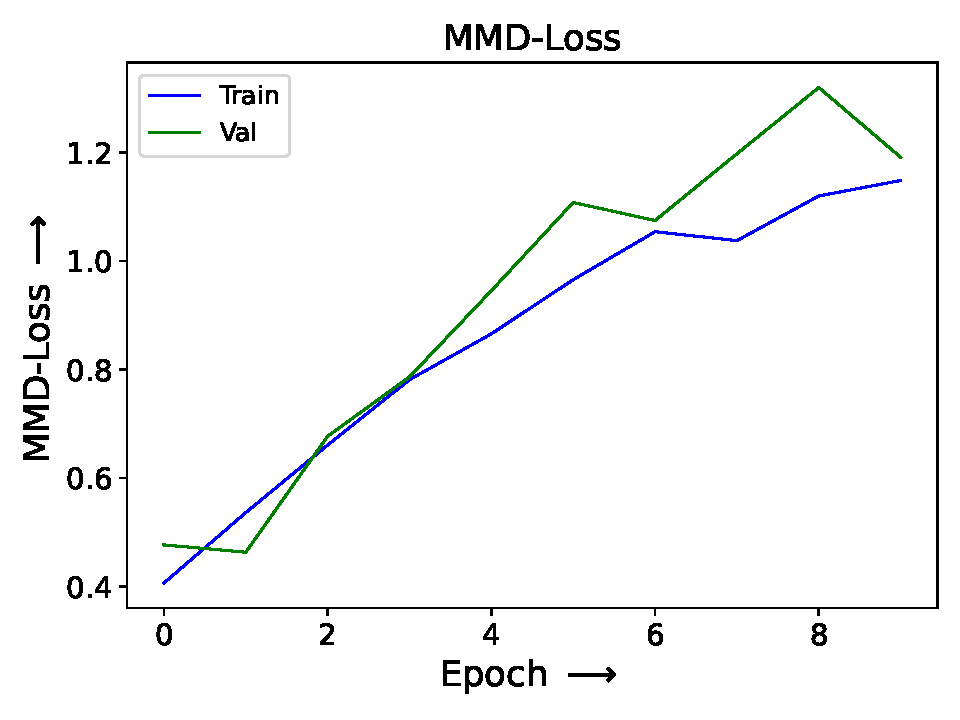
\includegraphics[width=.47\textwidth]{GAMMA_Influence_dummy_curve/MMD_Loss_GAMMA_0_001.pdf}
  \hspace{.3cm}
  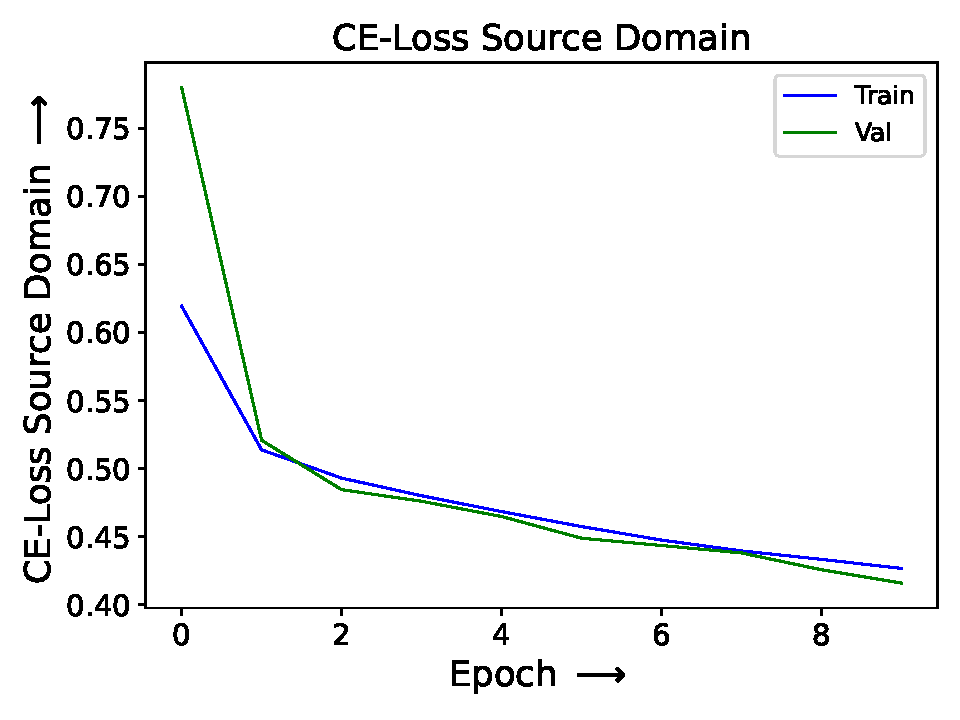
\includegraphics[width=.47\textwidth]{GAMMA_Influence_dummy_curve/CE_Loss_Source_Domain_GAMMA_0_001.pdf}

  \vspace{.1cm}

  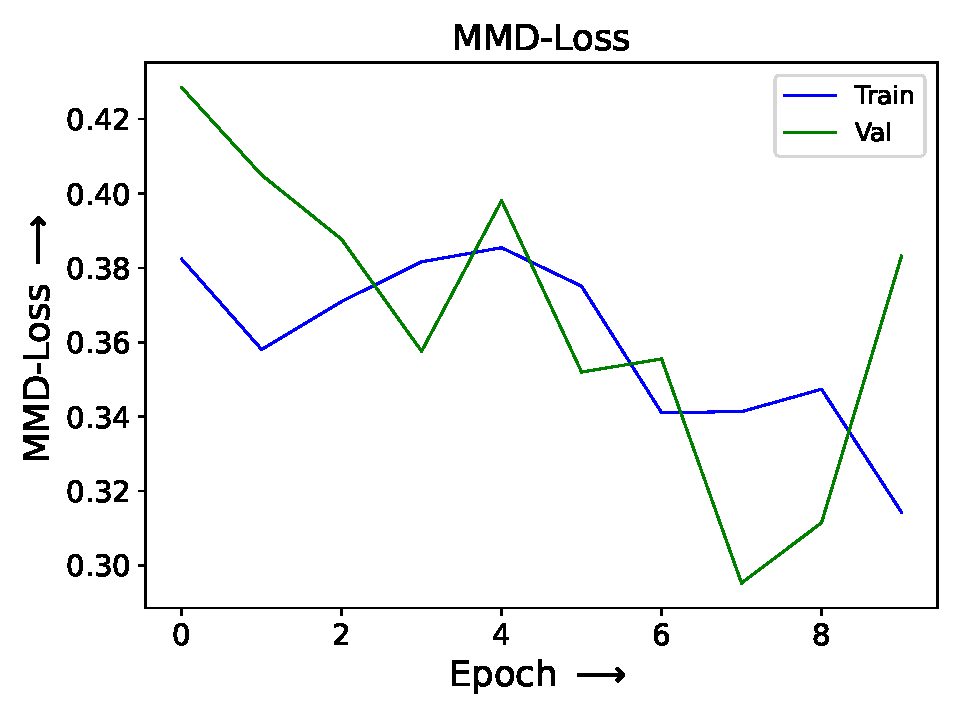
\includegraphics[width=.47\textwidth]{GAMMA_Influence_dummy_curve/MMD_Loss_GAMMA_0_1.pdf}
  \hspace{.3cm}
  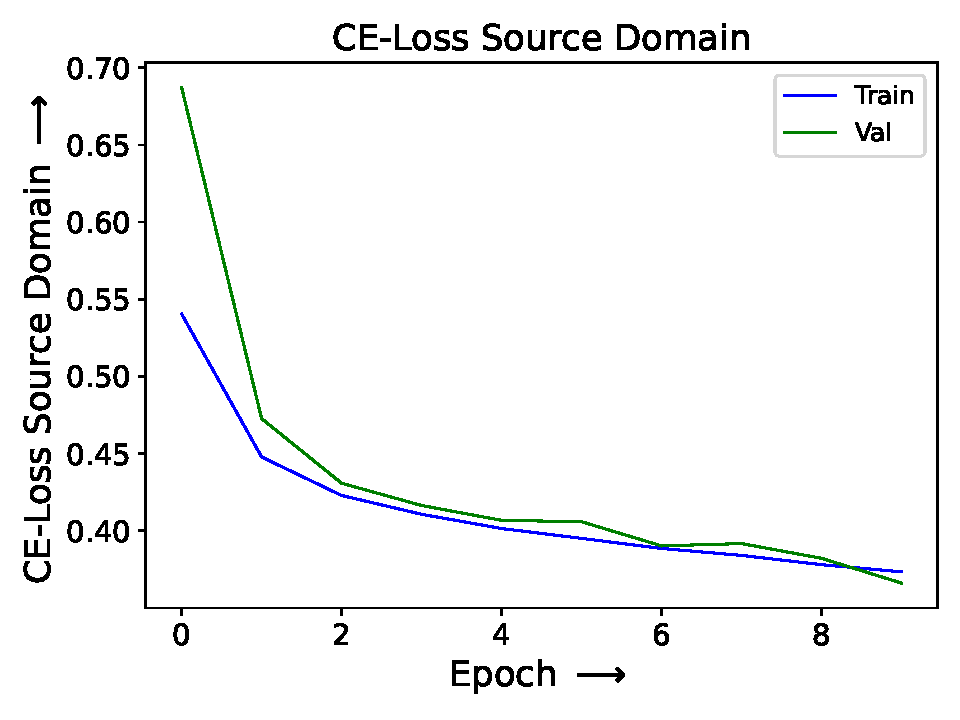
\includegraphics[width=.47\textwidth]{GAMMA_Influence_dummy_curve/CE_Loss_Source_Domain_GAMMA_0_1.pdf}

  \vspace{.1cm}

  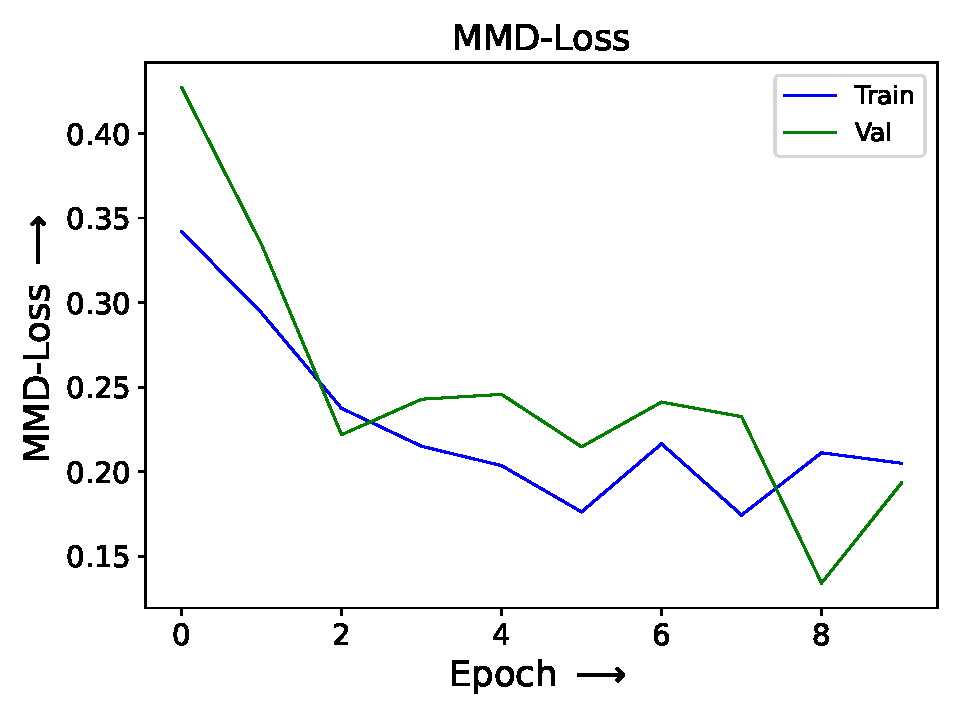
\includegraphics[width=.47\textwidth]{GAMMA_Influence_dummy_curve/MMD_Loss_GAMMA_20.pdf}
  \hspace{.1cm}
  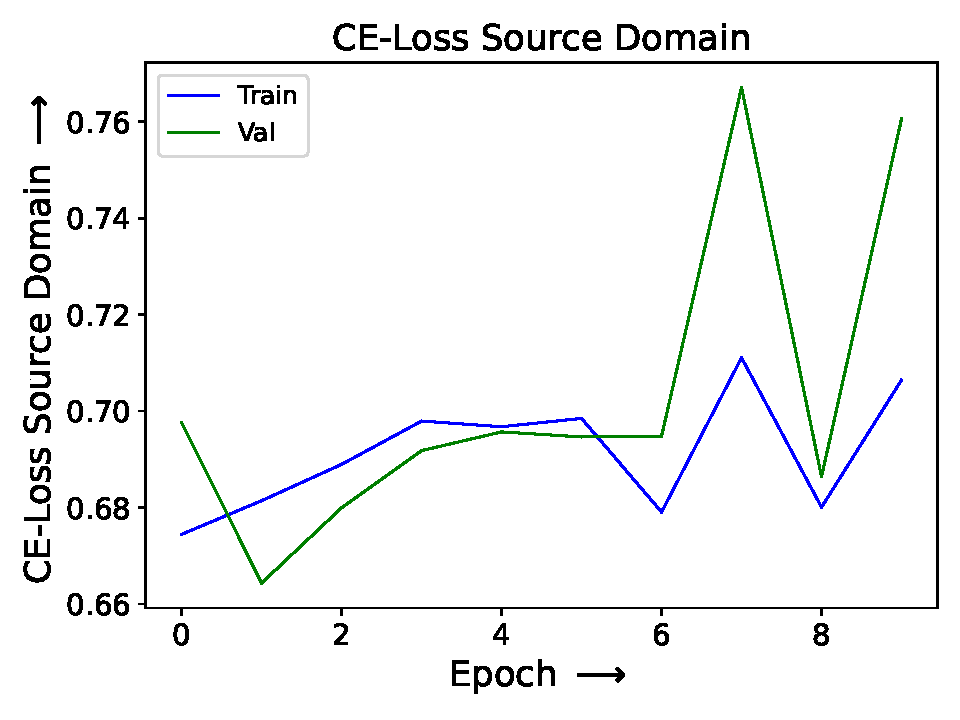
\includegraphics[width=.47\textwidth]{GAMMA_Influence_dummy_curve/CE_Loss_Source_Domain_GAMMA_20.pdf}

  \caption{MMD- and source CE-loss: Influence of the GAMMA choice on the model training: GAMMA = 0.001 (top), GAMMA = 0.1 (middle), GAMMA = 20 (bottom), Epoch 0 (left), Epoch 8 (right)}
  \label{fig:learning_curves_influence_mmd_feature_extractor}
\end{figure}

\subsection{Domain Adaptation Performance of the Labeled MMD-loss} \label{sec:Differences of labeled and unlabeled MMD loss}

In the literature, some approaches, like the one proposed by Pandhare et al. \cite{Pandhare2021}, extended the unlabeled MMD-based model training with a distance-based optimization, which included target labels. A novel labeled MMD-loss was developed in this thesis, which separately optimizes the domain discrepancy between the source and target domain samples of similar and different classes. When applying that MMD-loss type, the source CE-loss is still restricted to the source domain data.
\subsubsection{Description of Labeled MMD-loss}
The labeled MMD-loss minimizes the intra-class and maximizes the inter-class discrepancy between the domains. This enables a simultaneous improvement of the classes' separability and compactness. Additional hyperparameters are required, which need to be defined beforehand. The hyperparameters GAMMA\_Intra\_Class and GAMMA\_Inter\_Class balance the maximization of the inter-class domain discrepancy, the minimization of intra-class domain discrepancy and the reduction of the source CE-loss:

\begin{equation}
\begin{split}
    \mbox{Total Loss} = & \mbox{GAMMA\_Intra\_Class}  \cdot \mbox{MMD\_Loss\_Intra\_Class} - \\
                              &\mbox{GAMMA\_Inter\_Class} \cdot \mbox{MMD\_Loss\_Inter\_Class} + \mbox{CE\_Loss}.
\end{split}
\end{equation}

The MMD-loss, which includes target labels, is named "labeled MMD-loss" and the one restricted to the source labels is referred to as "unlabeled MMD-loss". Only target labels of 20\% of the target training samples were used in the labeled MMD-loss.

\subsubsection{Results of Labeled MMD-loss}
Figure \ref{fig:point_cloud_labeled_unlabeled_mmd}
visualizes the FC2 latent feature representations of the source and target domain samples during different epochs. Compared to the unlabeled MMD-loss, the labeled MMD-loss more efficiently reduced the domain discrepancy while increasing the separability and compactness of the classes in both domains. These improvements, achieved by the labeled MMD-loss, simplified the classification problem. The three advantages the labeled MMD-loss had over the unlabeled MMD-loss were proved by the following observations during the experiments (see figure \ref{fig:point_cloud_labeled_unlabeled_mmd}):
\begin{itemize}
    \item \textbf{Separability}: The distance between the classes was substantially increased and the separating subspace was less dense.
    \item \textbf{Compactness}: The samples belonging to the same class were represented in a more distinct subset. The distance of the samples to their corresponding class center was reduced. 
    \item \textbf{Domain Discrepancy}: The subsets corresponding to the same classes overlapped more across the domains.
\end{itemize}

In a  research aspect, the application of the labeled MMD-loss was interesting as it revealed the deficits of the unlabeled MMD-loss. Due to the lack of target labels, the unlabeled MMD-loss equally minimizes the intra- and inter-class domain discrepancy. Therefore, the unlabeled MMD-loss is more prone to minimizing the classes' separability while reducing the domain discrepancy. When the effect of the unlabeled MMD-loss becomes too dominant, the separability of the classes is destroyed. In this case, the optimization ends up in a trivial solution, in which the latent feature representations of all samples collapse to a point- or needle-like subspace. The GAMMA must be selected precisely to prevent that. Due to the separate optimization of the domain discrepancy between samples of equal and different classes, the model training with the labeled MMD-loss is less prone to the previously described trivial solution. Therefore, the dominance of the labeled MMD-loss can be increased during the optimization, which reduces the domain discrepancy more efficiently. This is also the reason, in this experiment, GAMMA\_Inter\_Class and GAMMA\_Intra\_Class were both chosen to be 30.


\begin{figure}[htp]
  \centering
  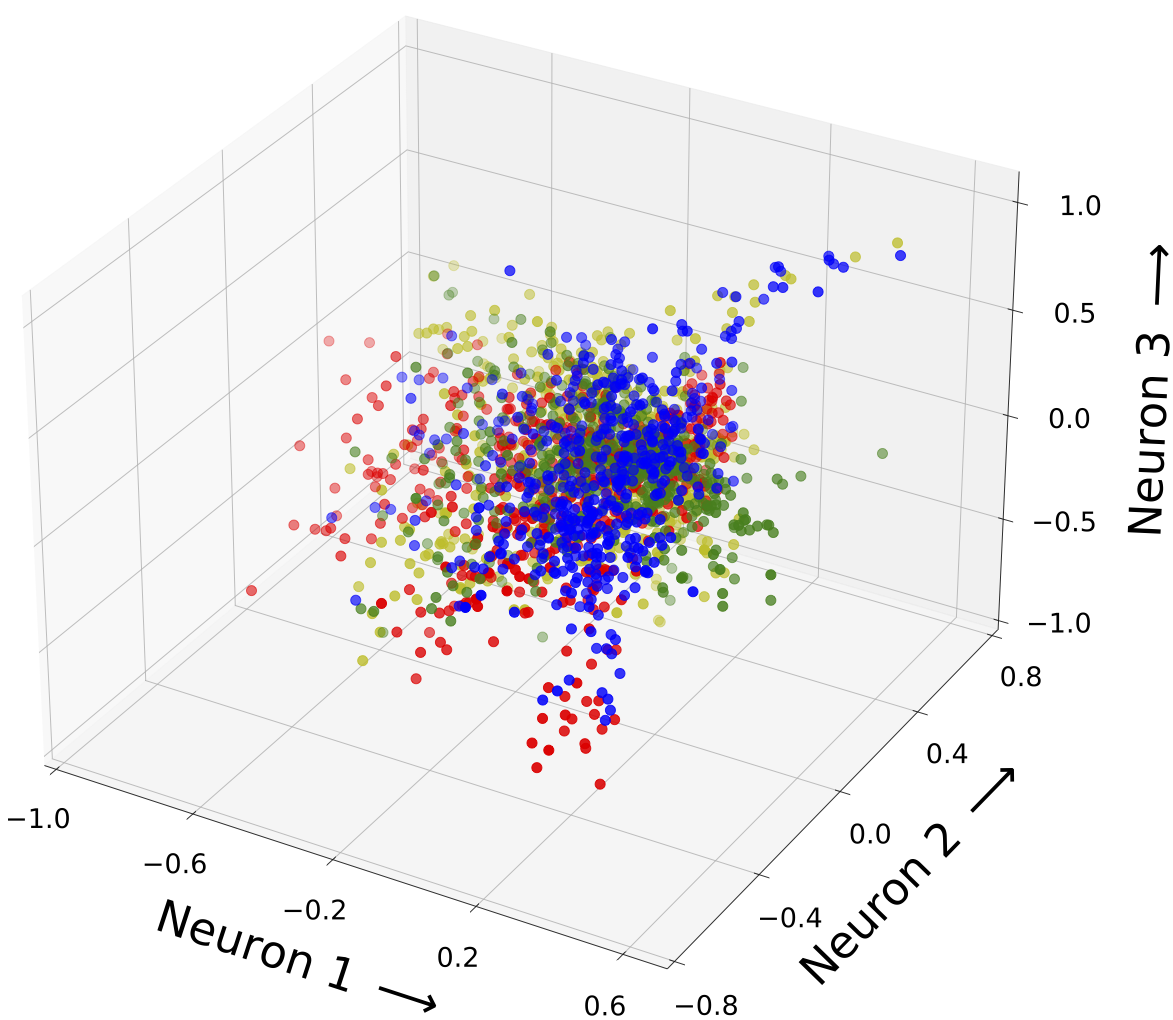
\includegraphics[width=.44\textwidth]{labeled_vs_unlabeled_point_cloud/data_distribution_labeled_mmd_0.png}
  \hspace{.4cm}
  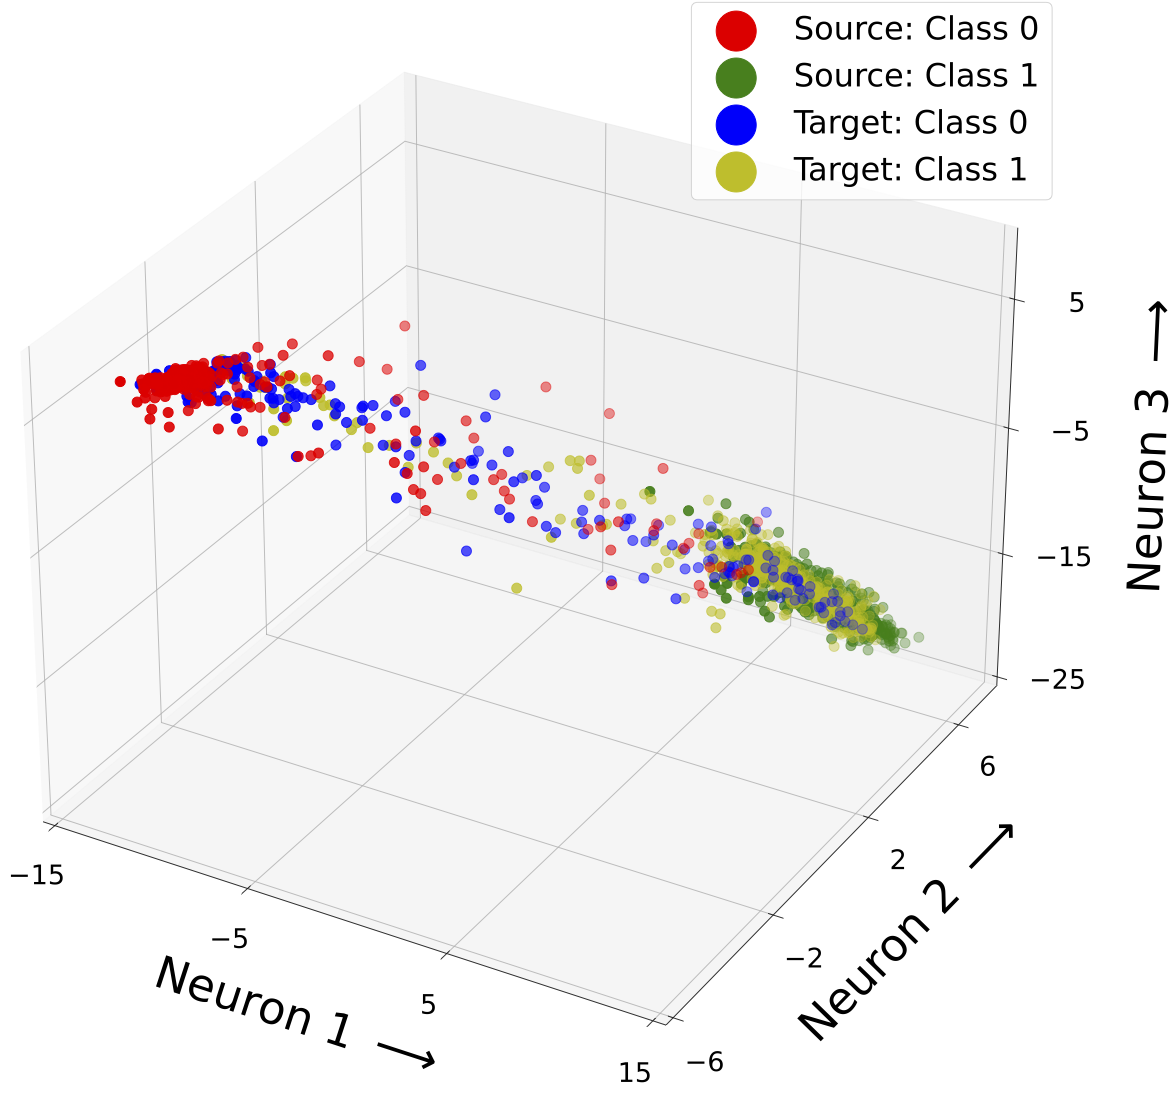
\includegraphics[width=.44\textwidth]{labeled_vs_unlabeled_point_cloud/data_distribution_labeled_mmd_8.png}

  \vspace{.1cm}

  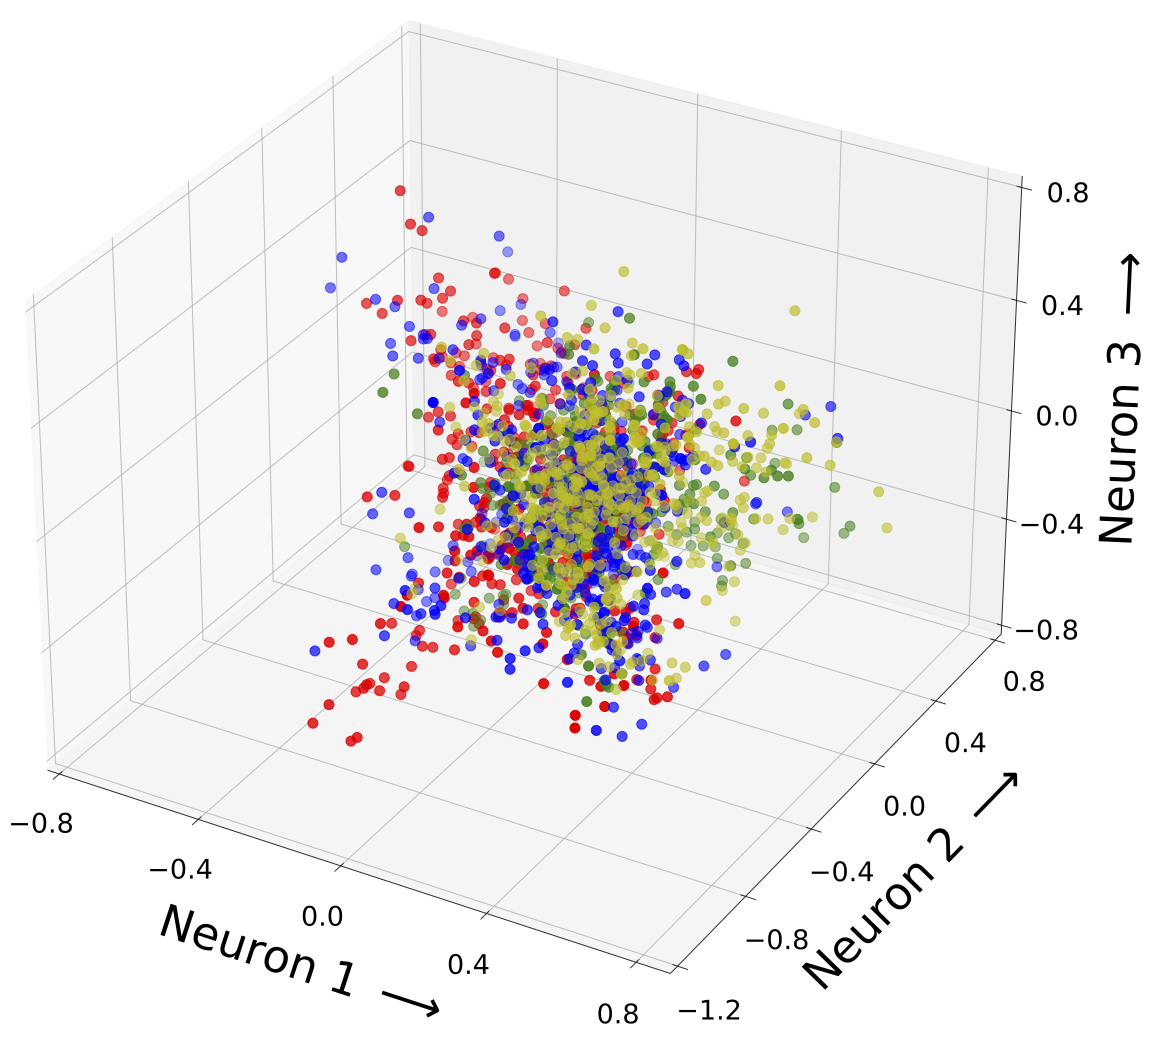
\includegraphics[width=.44\textwidth]{labeled_vs_unlabeled_point_cloud/data_distribution_regular_mmd_0.png}
  \hspace{.4cm}
  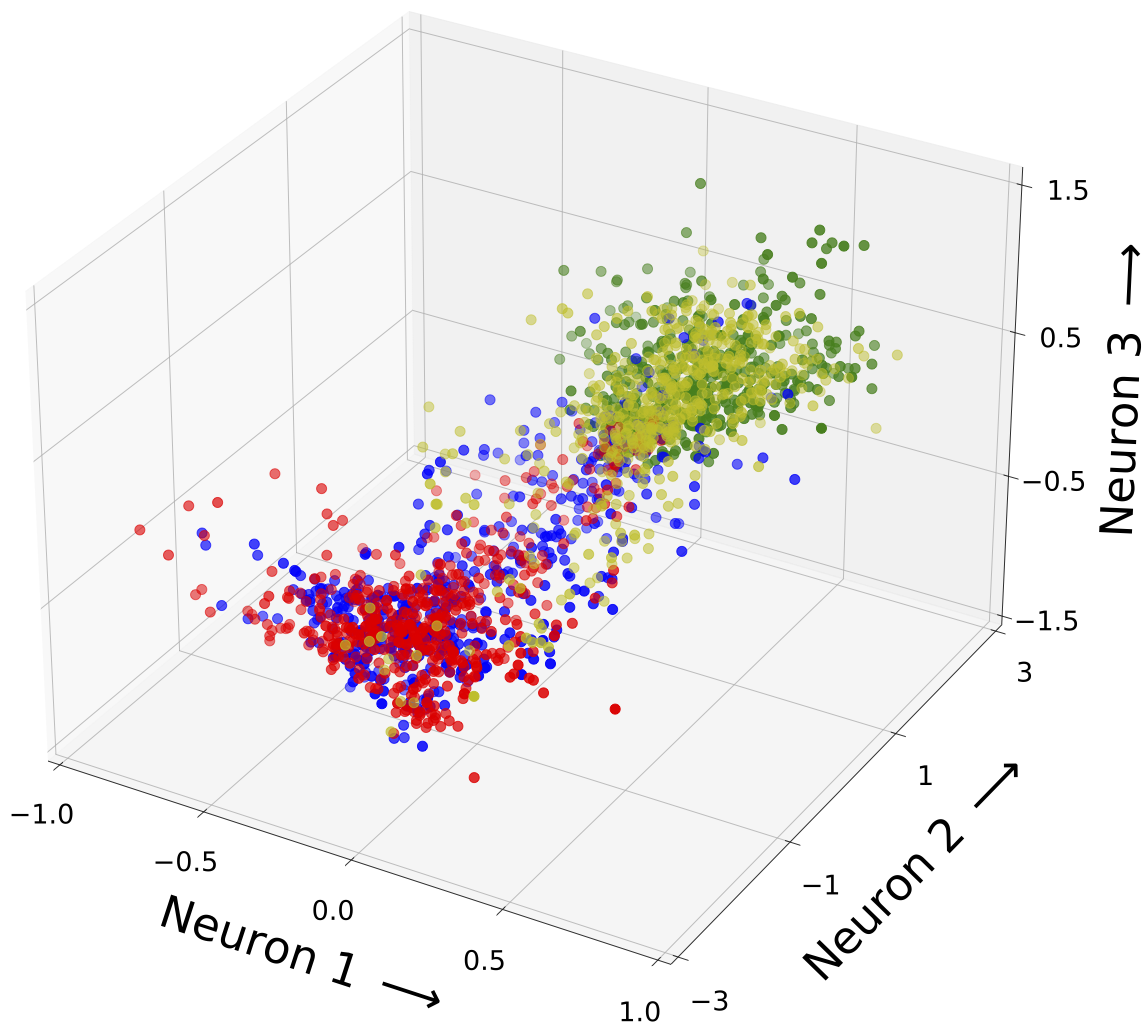
\includegraphics[width=.44\textwidth]{labeled_vs_unlabeled_point_cloud/data_distribution_regular_mmd_8.png}
  
  \caption{Data Distribution: Labeled MMD (top) vs. unlabeled MMD (bottom): Epoch 0 (left) vs. Epoch 8 (right)}
  \label{fig:point_cloud_labeled_unlabeled_mmd}
\end{figure}

\subsection{Influence of the Latent Feature Space Choice on the Domain Adaptation Performance}
\label{cnn_mmd_dummy}

This section analyzes how applying the MMD-loss in different latent feature maps of the CNN and classifier influences the model training. Inspired by Aljundi et al. \cite{Aljundi2016}, the domain discrepancy reduction in the CNN layers is investigated. Two different MMD-loss types were compared in experiments performed on the dummy dataset. Table \ref{tab:MMD_layer_choice_dummy} specifies the layers of the neural network considered by those MMD-loss types.

\begin {table}[H]
\centering

\begin{tabular}{llllllll}
  \toprule
  Model          & Conv1 & Conv2 & Conv3 & Flatten & FC1 & FC2 \\
  \midrule
  
 
\vspace{.5cm}

 \parbox[t]{0mm}{\multirow{1}{*}{\rotatebox[origin=c]{90}{\thead{FC \\ MMD}}}} & - & - & - & \checkmark & \checkmark & \checkmark\\
 
\vspace{.5cm}

 \parbox[t]{0mm}{\multirow{1}{*}{\rotatebox[origin=c]{90}{\thead{CNN \\ MMD}}}} & \checkmark & \checkmark & \checkmark & - & - & -\\

  \bottomrule
\end{tabular}

\caption {Overview of the latent feature maps included in the different MMD-loss types} \label{tab:MMD_layer_choice_dummy} 
\end {table}

The development of the source accuracy, target accuracy, source CE-loss and MMD-loss throughout the executed model training are visualized in figure \ref{fig:accuracy_cnn_and_no_cnn_mmd} and figure \ref{fig:loss_cnn_and_no_cnn_mmd}. When using the CNN feature maps in the MMD-loss, higher source and target accuracies were achieved. The domain discrepancy was reduced more efficiently by the CNN MMD-loss, which simplified the classification problem. Additionally, the losses converged faster and smoother. This proves the increased training stability when applying the MMD-loss in the CNN layers. When estimating the MMD-loss in the fully-connected layers, it seemed like the two contradicting training goals of the MMD- and source CE-loss worked against each other. In this case, the model training appeared to be more prone to get stuck in local minima. This was mainly reflected by the increasing training instabilities. The resulting fluctuations can be seen in the training curves. However, one has to remember that calculating the CNN MMD-loss is expensive, since the feature maps of the convolutional layers are complex and high-dimensional.

\begin{figure}[htp]
  \centering
  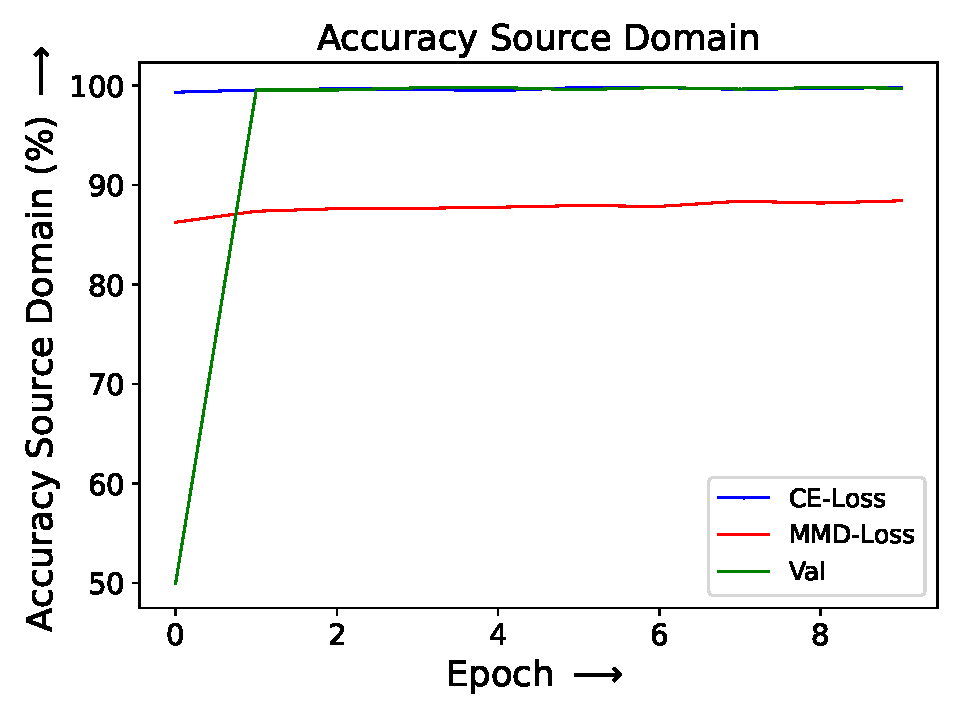
\includegraphics[width=.47\textwidth]{plots_CNN_MMD/Accuracy_Source_Domain_CNN_MMD.pdf}
  \hspace{.3cm}
  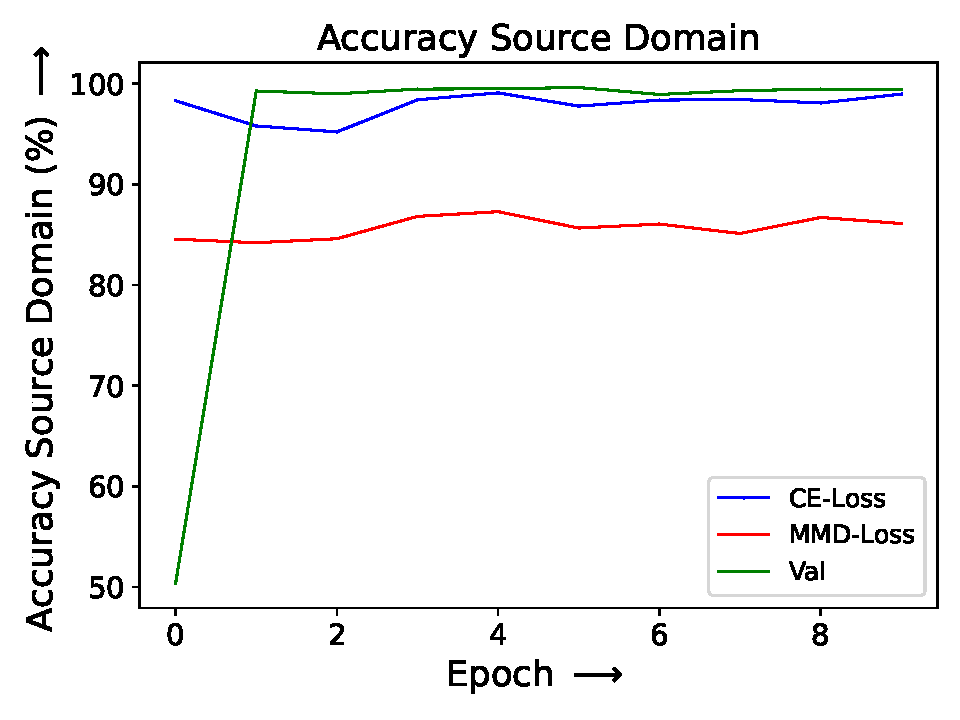
\includegraphics[width=.47\textwidth]{plots_CNN_MMD/Accuracy_Source_Domain_FC_MMD.pdf}

  \vspace{.1cm}

  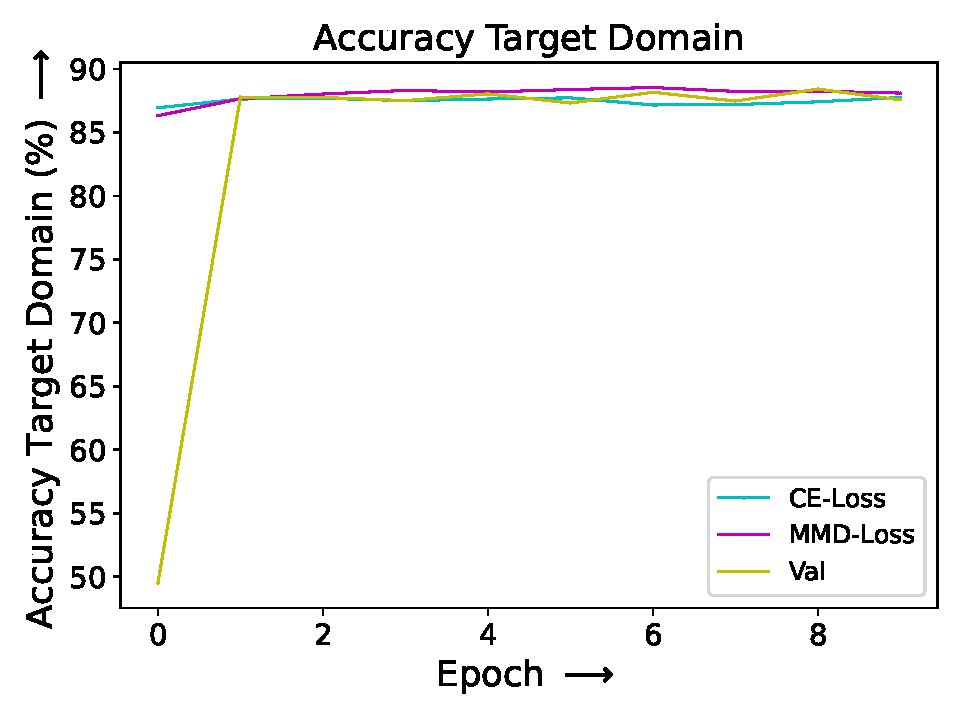
\includegraphics[width=.47\textwidth]{plots_CNN_MMD/Accuracy_Target_Domain_CNN_MMD.pdf}
  \hspace{.3cm}
  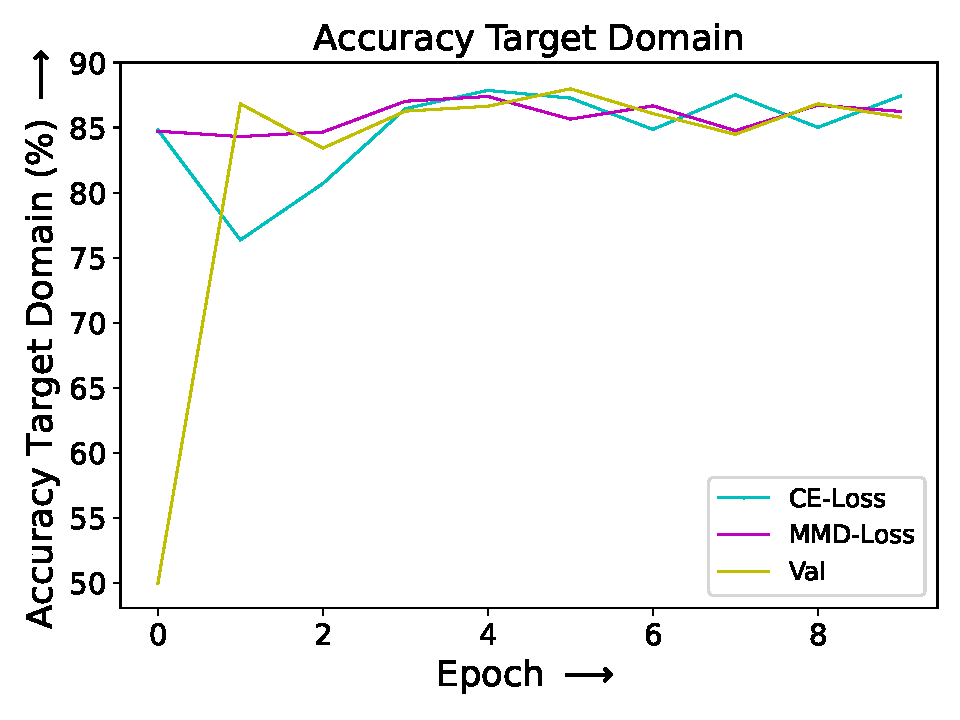
\includegraphics[width=.47\textwidth]{plots_CNN_MMD/Accuracy_Target_Domain_FC_MMD.pdf}

  \caption{Source and target accuracy: Influence of the MMD layer choice on the model training: CNN MMD (left), FC MMD (right)}
  \label{fig:accuracy_cnn_and_no_cnn_mmd}
\end{figure}

\begin{figure}[H]
  \centering
  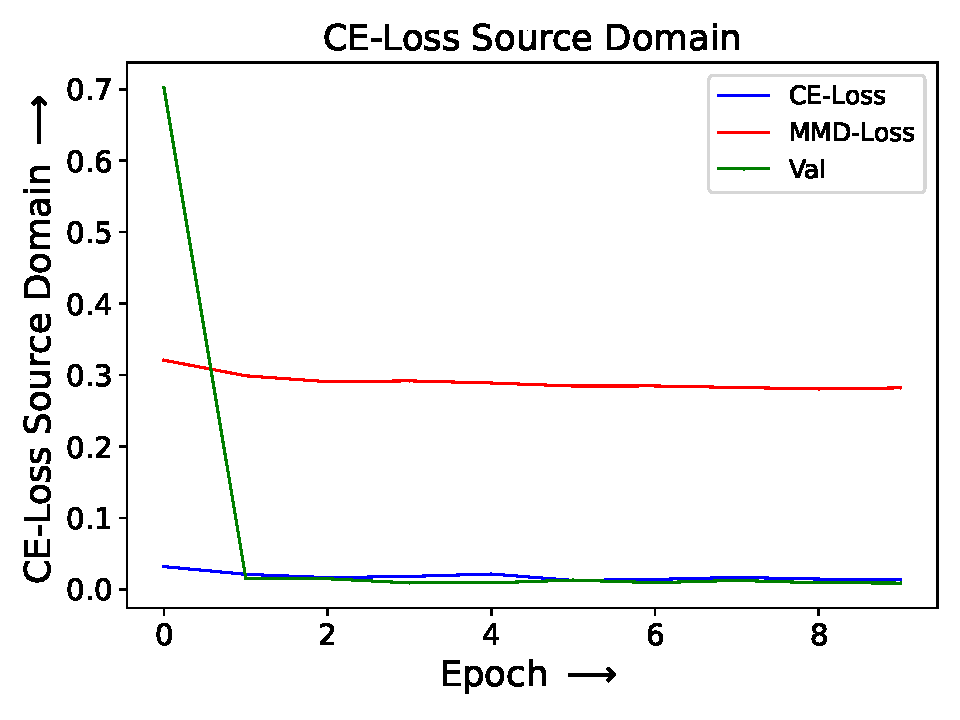
\includegraphics[width=.47\textwidth]{plots_CNN_MMD/CE_Loss_Source_Domain_CNN_MMD.pdf}
  \hspace{.3cm}
  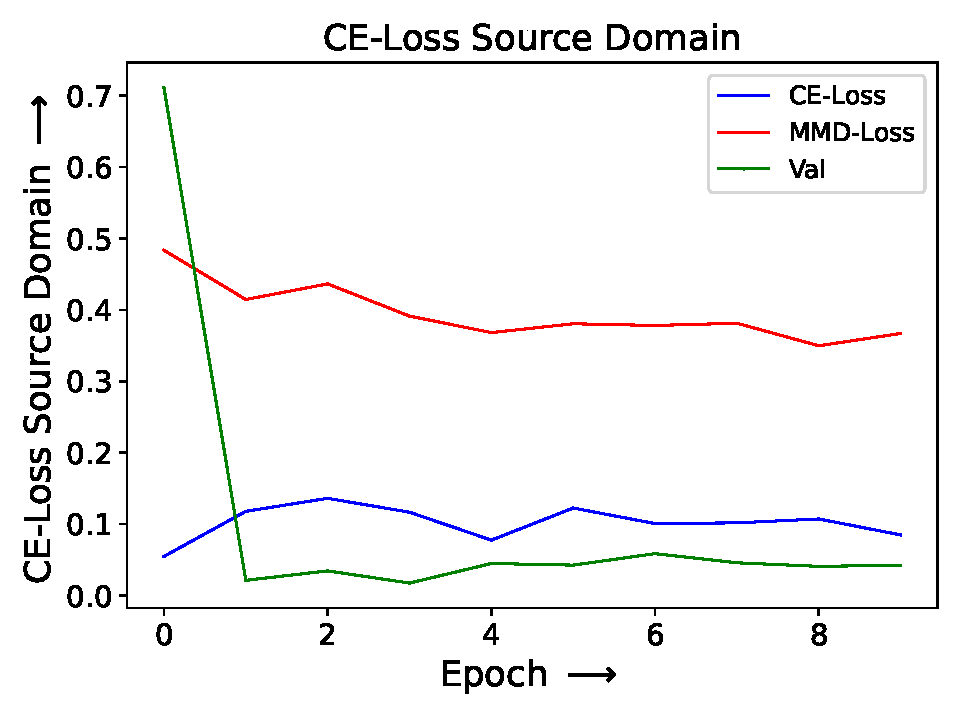
\includegraphics[width=.47\textwidth]{plots_CNN_MMD/CE_Loss_Source_Domain_FC_MMD.pdf}

  \vspace{.1cm}

  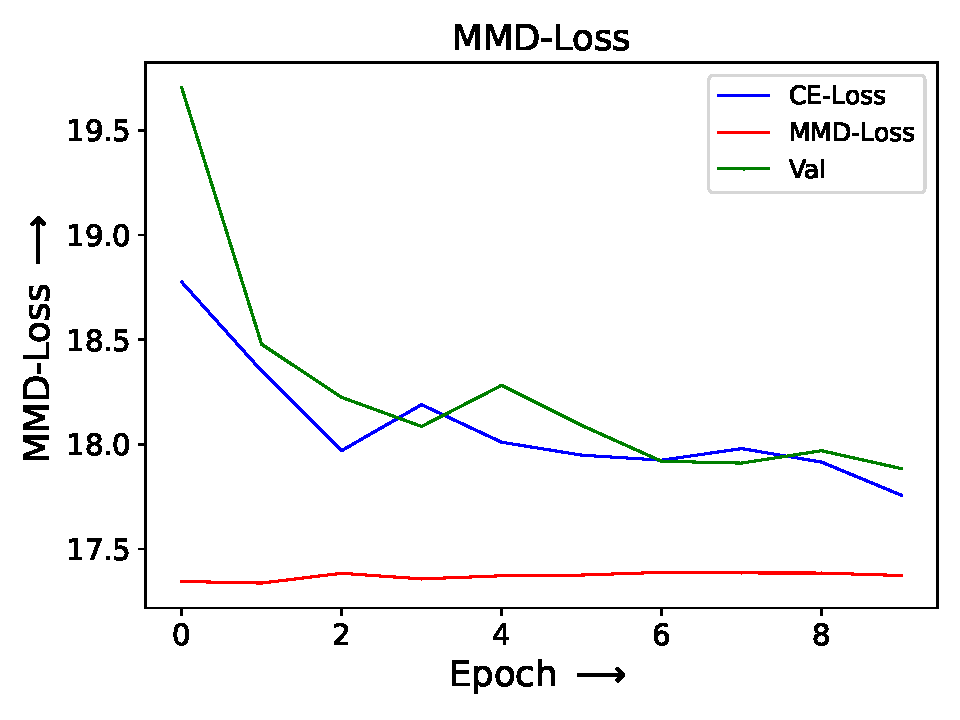
\includegraphics[width=.47\textwidth]{plots_CNN_MMD/MMD_Loss_CNN_MMD.pdf}
  \hspace{.1cm}
  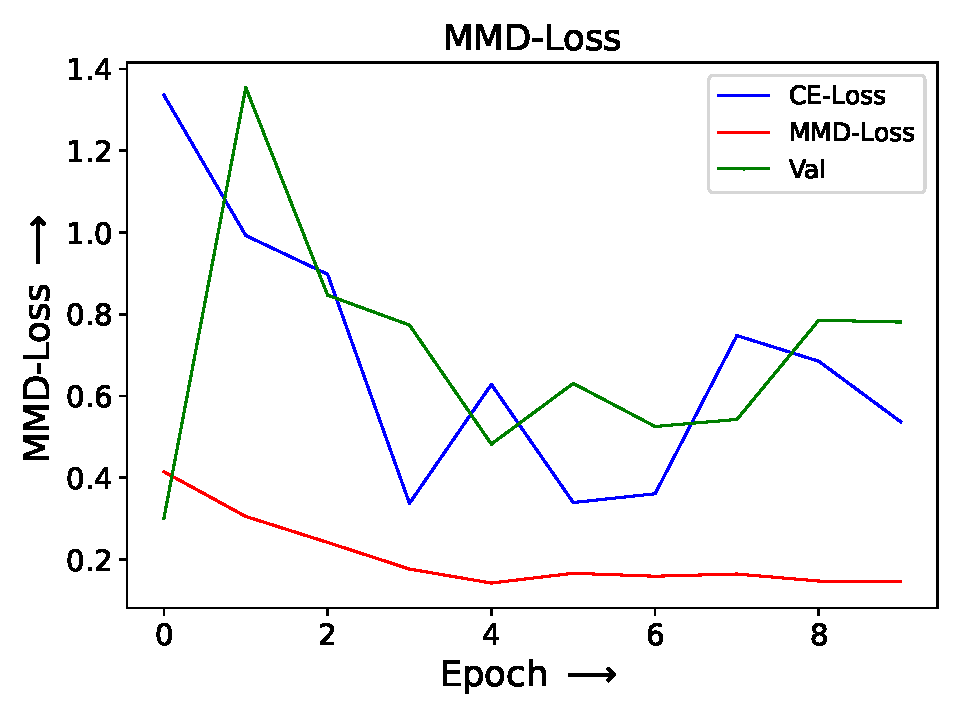
\includegraphics[width=.48\textwidth]{plots_CNN_MMD/MMD_Loss_FC_MMD.pdf}

  \caption{MMD- and Source CE-Loss: Influence of the MMD layer choice on the model training: CNN MMD (left), FC MMD (right)}
  \label{fig:loss_cnn_and_no_cnn_mmd}
\end{figure}

\section{Real-World Dataset}\label{sec:results_real_world_dataset}
In the following, the performance of models trained with different MMD-losses are evaluated on the real-world BSD dataset. The goal of this chapter is to investigate the benefits and problems of MMD-based domain adaptation for the PHM of industrial machines. All trained models had the same architecture and optimization strategy but differed in the applied MMD-losses. The evaluated MMD-losses differ in their GAMMA and latent feature space choices. The developed MMD-based models were compared with baseline models that did not apply any MMD-loss during the training. Table \ref{tab:MMD_layer_choice}  specifies the latent feature spaces included in the different applied MMD-loss types:

\begin {table}[H]
\centering

\begin{tabular}{llllllll}
  \toprule
  Model          & Conv1 & Conv2 & Conv3 & Flatten & FC1 & FC2 \\
  \midrule
  
\vspace{.5cm}

 \parbox[t]{0mm}{\multirow{1}{*}{\rotatebox[origin=c]{90}{\thead{BASE- \\ LINE}}}} & - & - & - & - & - & -\\
 
\vspace{.5cm}

 \parbox[t]{0mm}{\multirow{1}{*}{\rotatebox[origin=c]{90}{\thead{FULL \\ MMD}}}} & \checkmark & \checkmark & - & \checkmark & \checkmark & \checkmark\\
 
\vspace{.5cm}

 \parbox[t]{0mm}{\multirow{1}{*}{\rotatebox[origin=c]{90}{\thead{FC \\ MMD}}}} & - & - & - & \checkmark & \checkmark & \checkmark\\
 
\vspace{.5cm}

 \parbox[t]{0mm}{\multirow{1}{*}{\rotatebox[origin=c]{90}{\thead{CNN \\ MMD}}}} & \checkmark & \checkmark & \checkmark & - & - & -\\

 
  \bottomrule
\end{tabular}

\caption {Overview of the latent feature maps included in the different MMD-loss types} \label{tab:MMD_layer_choice} 
\end {table}

Similar to the dummy dataset, the influence of the GAMMA and latent feature space choice on the performance of the developed MMD-based PHM model are examined in chapters \ref{ch:Influence_GAMMA_real_dataset} and \ref{ch:Influence_Layer_real_dataset}. For several reasons, the previously presented labeled MMD-loss was excluded from this evaluation on the real-world BSD dataset. 
\begin{itemize}
    \item The labeled MMD-loss uses target labels, which no other MMD-loss type in this thesis does. To achieve good comparability only models with equal prerequisites and data access during the training are considered in this evaluation.
    \item Optimization methods using target labels are generally impractical for real-world use. In domain adaptation tasks, the neural networks are first trained on the source domain and afterward are transferred to the target domain. If the optimization methods require target labels, one could train the neural networks directly on the target domain. The necessity of target labels prevents the easy model adaptation by solely including the unlabeled target dataset in the model training. Labeling a dataset is often done manually and can be time-consuming.
    \item The labeled MMD-loss requires additional hyperparameters. Further experiments need to be executed to find those. The limited time in this thesis is also why the experiments on the real-world dataset are restricted to the unlabeled MMD-loss. 
\end{itemize}

Chapter \ref{ch:PHM_performance} compares the models based on their performance on the real-world BSD dataset. In chapter \ref{sec:Performance_overview}, the results from the dummy and real-world dataset are concluded. All computations were performed on a Leibniz Supercomputing Centre7 compute node virtual machine with 20 Intel® Xeon® Gold 6148 vCPUs, one Nvidia® Tesla V100, 368 GB RAM, PyTorch v.1.4.0 and CUDA 10.1.


\subsection{Influence of the GAMMA Choice on the PHM Performance}\label{ch:Influence_GAMMA_real_dataset}

Three models were trained with the FULL MMD-loss and different GAMMAs (0, 0.05, 1) on the D:P mech./X signal for 100 epochs. Figure \ref{fig:distribution_GAMMA_influence_real_data} 
shows the FC2 latent feature representations of the source and target domain samples during
different epochs. Similar to the dummy dataset, the MMD-based model training was highly sensitive to the GAMMA choice. When GAMMA was selected precisely, the domain discrepancy was reduced, while guaranteeing sufficient compactness and separability of the classes in the source and target domain. For the given PHM task, the GAMMA choice of 0.05 was suitable, which is prooved by the following observations:
\begin{itemize}
    \item \textbf{Separability}: The structure of the data distribution offered the greatest clarity and smoothness. This raised the assumption that separating the classes in this latent feature space data distribution was less complex. 
    \item \textbf{Compactness}: Class 1 appeared to be more compact in both domains. All samples lay in a more distinct subspace with a decreased distance to the corresponding class center.
    \item \textbf{Domain Discrepancy}: The target domain samples of class 0 appeared to be less mixed with the source and target domain samples belonging to class 1. 
\end{itemize}

However, it is difficult to compare the separability, compactness and domain overlap of the classes from the plots. Nevertheless, the plots make the disadvantages of choosing a GAMMA of 1 very obvious. In this case, the MMD-loss was too dominant. Noise and unimportant information were transferred between the domains. The MMD-loss reduced the distance between the source and target samples of all classes. This destroyed the class structure of the source and target domain. In this case, the feature representations of all samples collapsed to a small needle-like subspace, which made the classification task impossible.

\begin{figure}[H]
  \centering
  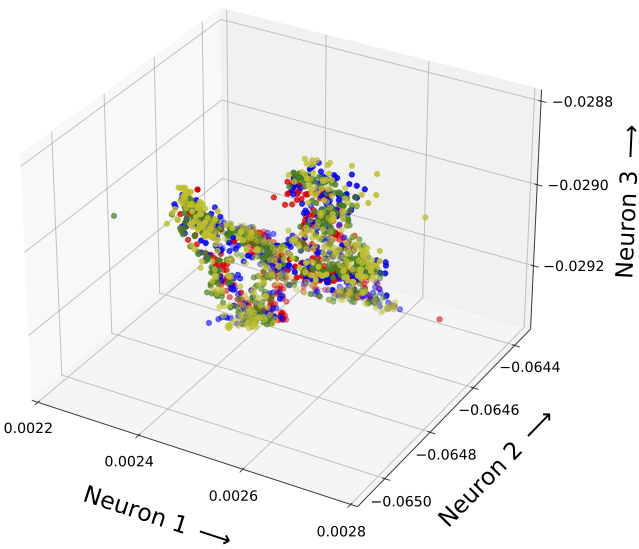
\includegraphics[width=.47\textwidth]{GAMMA_Influence_real_data/P_mech_X_data_distribution_0_GAMMA_0_0.png}
  \hspace{.4cm}
  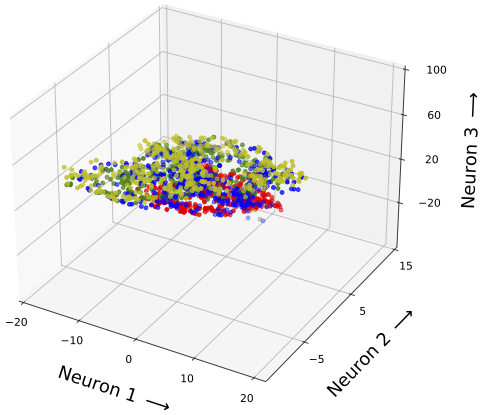
\includegraphics[width=.47\textwidth]{GAMMA_Influence_real_data/P_mech_X_data_distribution_80_GAMMA_0_0.png}

  \vspace{.1cm}

  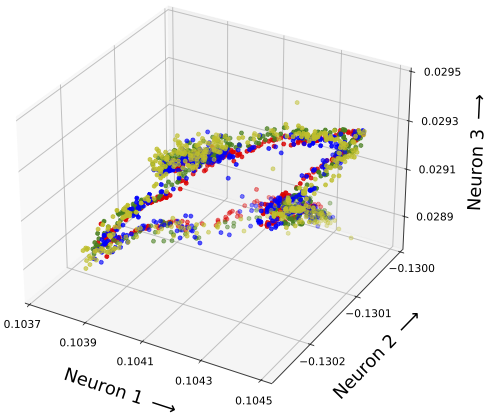
\includegraphics[width=.47\textwidth]{GAMMA_Influence_real_data/P_mech_X_data_distribution_0_GAMMA_0_05.png}
  \hspace{.4cm}
  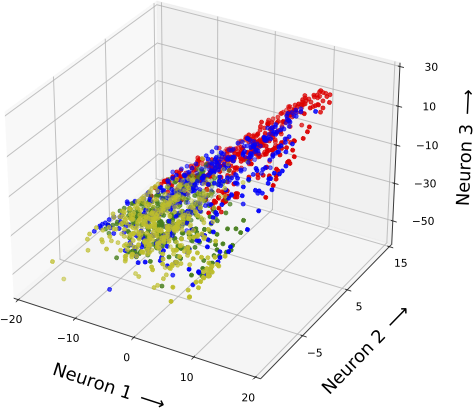
\includegraphics[width=.47\textwidth]{GAMMA_Influence_real_data/P_mech_X_data_distribution_80_GAMMA_0_05.png}

  \vspace{.1cm}

  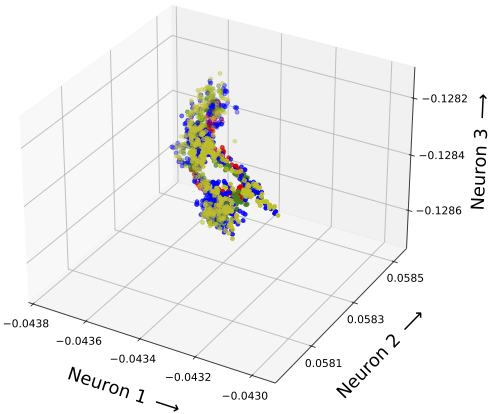
\includegraphics[width=.47\textwidth]{GAMMA_Influence_real_data/P_mech_X_data_distribution_0_GAMMA_1_0.png}
  \hspace{.4cm}
  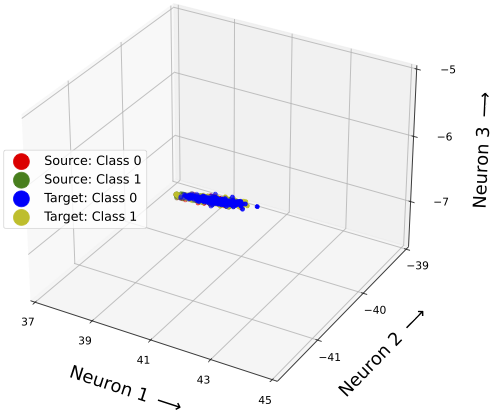
\includegraphics[width=.47\textwidth]{GAMMA_Influence_real_data/P_mech_X_data_distribution_80_GAMMA_1_0.png}

  \vspace{.1cm}

  \caption{Data  distribution:  Influence of the GAMMA choice on the model training:  GAMMA  =  0  (top), GAMMA = 0.05 (middle), GAMMA = 1 (bottom), Epoch 0 (left), Epoch 100 (right)}
  \label{fig:distribution_GAMMA_influence_real_data}
\end{figure}


\subsection{Influence of the Latent Feature Space Choice on the PHM Performance}\label{ch:Influence_Layer_real_dataset}
This section analyzes the effects of different latent feature space choices on the MMD-based model training. All models were trained with a GAMMA of 1 on the D:I soll/X signal for 100 epochs. Each model training was repeated five times in an equal matter. Figure \ref{fig:target_accuracy_MMD_layer} shows the corresponding target accuracy development during the executed training. When the MMD-loss was solely applied in the FC layers, the training collapsed in two of the five experiments (row 3, 5). In the other three cases, the accuracy had a slight tendency to decrease during the training. The CNN MMD-based model training showed worse reproducibility throughout the five experiments than the FULL MMD-based model training. Often, the fluctuations on the validation data were not reduced properly throughout the training (row 1, 4, 5). The FULL MMD-based model training appeared to be more stable, especially towards the end of the training. Nevertheless, minor fluctuations were also observable for the FULL MMD-based model training (row 3, 4). In this thesis, the final model was selected based on its performance on the validation dataset of the target domain. In real-world scenarios, the target labels are usually unknown. Often, the model at the end of the training is chosen as the final one. When the model performance decreases or fluctuates throughout the training, the best possible model is unlikely to be found. For this reason, a stable and converging model training is important for real-world applications. A more detailed description of how the final models are chosen is given in chapter \ref{ch:PHM_performance}. 

\begin{figure}[H]
  \centering

  \includegraphics[width=.32\textwidth]{MMD_LAYER_influence_real_data/CNN_MMD/Accuracy_Target_Domain_1.pdf}
  \hspace{.1cm}
  \includegraphics[width=.32\textwidth]{MMD_LAYER_influence_real_data/FC_MMD/Accuracy_Target_Domain_1.pdf}
  \hspace{.1cm}
  \includegraphics[width=.32\textwidth]{MMD_LAYER_influence_real_data/FULL_MMD/Accuracy_Target_Domain_1.pdf}

  \vspace{.3cm}

  \includegraphics[width=.32\textwidth]{MMD_LAYER_influence_real_data/CNN_MMD/Accuracy_Target_Domain_2.pdf}
  \hspace{.1cm}
  \includegraphics[width=.32\textwidth]{MMD_LAYER_influence_real_data/FC_MMD/Accuracy_Target_Domain_2.pdf}
  \hspace{.1cm}
  \includegraphics[width=.32\textwidth]{MMD_LAYER_influence_real_data/FULL_MMD/Accuracy_Target_Domain_2.pdf}

  \vspace{.3cm}

  \includegraphics[width=.32\textwidth]{MMD_LAYER_influence_real_data/CNN_MMD/Accuracy_Target_Domain_3.pdf}
  \hspace{.1cm}
  \includegraphics[width=.32\textwidth]{MMD_LAYER_influence_real_data/FC_MMD/Accuracy_Target_Domain_3.pdf}
  \hspace{.1cm}
  \includegraphics[width=.32\textwidth]{MMD_LAYER_influence_real_data/FULL_MMD/Accuracy_Target_Domain_3.pdf}
  
    \vspace{.3cm}

  \includegraphics[width=.32\textwidth]{MMD_LAYER_influence_real_data/CNN_MMD/Accuracy_Target_Domain_4.pdf}
  \hspace{.1cm}
  \includegraphics[width=.32\textwidth]{MMD_LAYER_influence_real_data/FC_MMD/Accuracy_Target_Domain_4.pdf}
  \hspace{.1cm}
  \includegraphics[width=.32\textwidth]{MMD_LAYER_influence_real_data/FULL_MMD/Accuracy_Target_Domain_4.pdf}
  
    \vspace{.3cm}
    
  \includegraphics[width=.32\textwidth]{MMD_LAYER_influence_real_data/CNN_MMD/Accuracy_Target_Domain_5.pdf}
  \hspace{.1cm}
  \includegraphics[width=.32\textwidth]{MMD_LAYER_influence_real_data/FC_MMD/Accuracy_Target_Domain_5.pdf}
  \hspace{.1cm}
  \includegraphics[width=.32\textwidth]{MMD_LAYER_influence_real_data/FULL_MMD/Accuracy_Target_Domain_5.pdf}


  \caption{Target accuracy: Influence of the MMD layer choice on the model training: CNN MMD (left), FC MMD (middle), FULL MMD (right)}
  \label{fig:target_accuracy_MMD_layer}
\end{figure}


\section{Overall PHM Performance}\label{ch:PHM_performance}
In this chapter, different MMD-loss types are evaluated on the real-world BSD dataset. This is done by comparing the performance of models trained with those MMD-loss types. The performance is measured by the models' accuracy on the target domain test dataset. The evaluation of the MMD-loss types required several stages of experiments.
In the first stage, all of the 49 signals were evaluated by their suitability for PHM tasks. The models were trained on these signals without applying any MMD-loss. Based on the performance of the resulting models, seven promising signals were selected for further testing. In the second stage, the models were optimized with different MMD-based training strategies on those seven signals. The models were optimized with FULL MMD-, FC MMD- and CNN MMD-losses and three different GAMMA choices (0.05, 0.5, 1). All nine MMD-based model training (all combinations of MMD types and GAMMAs) and the baseline model training that did not apply any MMD-loss were repeated five times on all seven signals. During each epoch in the model training, the models were evaluated based on the balanced accuracy on the target domain validation dataset and the best-performing model was stored. The different MMD-loss types were compared by the performance of those stored models on the unseen target domain test dataset.



For each training strategy, the accuracies of five models optimized in equally repeated training were averaged. The results are shown in table \ref{tab:Mean_Accuracy}. The FULL MMD models performed best on four of the seven signals and the CNN MMD models on the other three. The FC MMD models never outperformed the other MMD-based models. Compared to the baseline model, the MMD-based models increased the accuracy by up to 10.18$\%$. Table \ref{tab:Variance_Accuracy} shows the standard deviations corresponding to the averaged accuracies seen in table \ref{tab:Mean_Accuracy}. The best-performing models usually showed low to average standard deviations, which verified a high degree of reproducibility throughout the repeated model training. This demonstrates the relevance of the results and proves the applicability and utility of the corresponding MMD-losses for reducing the domain discrepancy in the PHM task. For all training strategies (BASELINE, FULL MMD, FC MMD, CNN MMD) the calculated standard deviations were averaged in the last column of table \ref{tab:Variance_Accuracy}. For the MMD-based model training, the average standard deviations were calculated over all signals and GAMMAs and for the baseline model training over all signals. From the MMD-based models, the FULL MMD models had the lowest average standard deviation and the FC MMD models had the highest. This proved that the FULL MMD models achieved the most consistent performance throughout repeated training with different GAMMAs and on different signals. The FULL MMD models were more robust and less sensible to GAMMA and signal choices. As mentioned in the results of the dummy dataset, a reason for the sensitivity of the FC MMD model training might be from the contradicting training goals when evaluating the MMD- and the source CE-loss solely in the FC layers. The training is possibly more prone to getting stuck in local minima, which leads to instabilities during the optimization.
\begin{comment}
Windowing functions split the recorded data in shorter sequences. The generated windows should capture the degradation related patterns of the vibration signals. For this reason, the windows should be adapted according to the consistency and periodicity of the data. In this thesis a window size of 1024 was chosen. The windowing requirements are different for the different machine excitements (constant speed excitement, direction change excitement and sweep excitement). The windows are too short to capture one whole period of of forward and backward motion in the data recorded during constant speed machine excitement. The data can be separated in phases of constant speed and direction change, which each contains roughly 1000 datapoints. The windows are of equal size as the described phases in the data. Since the windows are not synchronized with those phases, they overlap to a large extent but do not cover them perfectly. The windows are big enough to capture several periods of forward and backward movements in data recorded during direction change excitement. When exciting the machine with a sweep signal the PHM system should better process the whole corresponding vibration signal. It is important to capture the changing frequencies and amplitudes during the complete sweep excitement. The best PHM results were achieved on data recorded during constant speed and  direction change excitement of the machine. This shows that the windowing did not work very well on the data recorded during sweep excitement. Generally, when choosing the window size, there is a trade-off between the window size and the number of windows generated from the data. Both extremes (few big windows and numerous small windows) might lead to problems during the training. The PHM results can probably be improved by an intelligent and adaptive preprocessing to generate suitable and synchronized data windows. Azamfat et al \cite{AZAMFAR2020103932} present such an approach. They apply a constant excitement to the machine and separate the data BSD phases of constant velocity direction change movement. The PHM system just relies on the data recorded during BSD constant velocity. The signals D:I\_ist/X (actual electrical power), D:I\_soll/X (target electrical power) and D:P\_mech./X (mechanical power) coming from the controller show high potential for the PHM task. The most suitable accelerometer installation is the one on the BSD nut. Pandahare et al \cite{Pandhare2021} discovered similar results. Often in real operational scenarios such an installation is impractical \cite{Pandhare2021}. Alternatively to the BSD nut position, this thesis shows, that the top LGS achieves better PHM results than the bottom one.
\end{comment}


\begin{sidewaystable}
%\begin{table}
\centering
\begin{tabular}{llllllllll}
  \toprule
  Model          & GAMMA    & D:I\_ist/X & D:I\_soll/X & D:P\_mech./X & C:z\_top & C:z\_nut & D:x\_nut & D:z\_top \\
  \midrule
  
  \vspace{1cm}
  
    \thead{BASE- \\ LINE}  & -      & 70.08 & 75.62 & 74.7 & 69.14 & 57.4 & 58.74 & 57.88\\


 
                            & 0.05   & 71.56 & 75.42 & \textbf{78.96} & 72.36 & 58.10 & 49.52 & \textbf{62,64}\\
    \thead{FULL \\ MMD}     & 0.5    & 73.78 & 74.84 & 52.78 & \textbf{75.92} & \textbf{64.76} & 50.52 & 49,94\\
    
    \vspace{1cm}
    
                            & 1      & 72.98 & 75.18 & 49.80 & 74.12 & 57.02 & 50.62 & 50.52\\


                            & 0.05   & 73.60 & 76.38 & 74.98 & 71.36 & 57.48 & 52.44 & 61.3\\
    \thead{FC \\ MMD}       & 0.5    & 70.74 & 74.86 & 72.62 & 69.32 & 59.76 & 50.12 & 53.22\\
    
    \vspace{1cm}
    
                            & 1      & 73.42 & 65.46 & 76.96 & 62.34 & 58.86 & 50.92 & 53.96\\

                            & 0.05   & 71.62 & \textbf{76.44} & 51.80 & 73.20 & 59.30 & 58.04 & 53.82\\
    \thead{CNN \\ MMD}      & 0.5    & \textbf{73.90} & 75.86 & 51.58 & 72.28 & 55.76 & 68.04 & 51.72\\
                            & 1      & 73.80 & 73.82 & 51.12 & 72.18 & 54.28 & \textbf{68.92} & 51.28\\
 \addlinespace
 \hline
 \thead{MMD\\GAIN:} &  & +3.82 & +0.82 & +4.26 & +6.78 & +7.36 & +10.18 & +4.76\\
 
  \bottomrule
\end{tabular}
\caption{Average target test accuracy (\%)} \label{tab:Mean_Accuracy} 
%\end{table}
\end{sidewaystable}

\begin{sidewaystable}
%\begin{table}
\centering
\begin{tabular}{lllllllllll}
  \toprule
  Model          & GAMMA    & D:I\_ist/X & D:I\_soll/X & D:P\_mech./X & C:z\_top & C:z\_nut & D:x\_nut & D:z\_top & AVG STD  \\
  \midrule

    \vspace{1cm}

    \thead{BASE- \\ LINE}   & -      & 2.07 & 0.27 & 2.20 & 2.55 & 1.11 & 1.04 & 1.22 & 1.50\\
 
                            & 0.05   & 1.06 & 0.74 & \textbf{1.79} & 1.80 & 2.04 & 1.39 & \textbf{2.48} & \\
    \thead{FULL \\ MMD}     & 0.5    & 0.72 & 1.44 & 3.33 & \textbf{1.72} & \textbf{1.42} & 1.23 & 1.02 & 1.81\\
    
    \vspace{1cm}  
    
                            & 1      & 0.76 & 0.81 & 0.87 & 6.06 & 5.57 & 0.96 & 0.79 & \\



                            & 0.05   & 1.96 & 0.61 & 1.86 & 1.82 & 1.63 & 3.86 & 1.60 & \\
    \thead{FC \\ MMD}       & 0.5    & 1.34 & 0.72 & 11.06 & 6.42 & 2.28 & 0.45 & 3.14 & 3.39\\
    
    \vspace{1cm}
    
                            & 1      & 0.96 & 12.01 & 5.46 & 8.18 & 2.13 & 0.93 & 2.70 & \\
                            & 0.05   & 2.13 & \textbf{0.53} & 2.39 & 1.12 & 4.01 & 4.18 & 7.26 & \\
    \thead{CNN \\ MMD}      & 0.5    & \textbf{0.25} & 1.57 & 1.08 & 1.22 & 3.27 & 3.51 & 3.22 & 2.45\\
                            & 1      & 0.51 & 1.25 & 2.02 & 2.51 & 4.54 & \textbf{2.54} & 2.34 & \\
  \bottomrule
\end{tabular}
\caption{Standard deviation target test accuracy (\%)} \label{tab:Variance_Accuracy} 
%\end{table}
\end{sidewaystable}


\section{Conclusion of the Experimental Results}\label{sec:Performance_overview}
In this chapter, the results from the experiments on the dummy and real-world datasets are interpreted and the corresponding findings are summarized. Variations in the underlying functionalities and mechanisms of the MMD-loss types became especially visible in the experiments on the dummy dataset. Performance differences between the MMD-loss types were evaluated on the real-world dataset. A novel labeled MMD-loss was developed, which considers the source and target labels. When applying the labeled MMD-loss, the domain discrepancy is reduced between the samples of the same class and increased between those of different classes. This guarantees improved compactness and separability of all classes while reducing the domain discrepancy. The experiments with the labeled MMD-loss on the dummy dataset highlighted the deficits of the unlabeled MMD-loss. Since the unlabeled MMD-loss has no access to the target labels, class-specific properties like the compactness and separability can not be optimized for the target domain. The unlabeled MMD-loss reduces the domain discrepancy between all samples without considering their class labels. If the unlabeled MMD-loss becomes too dominant, the separability of the classes is reduced and the data structure is destroyed. In this case, the latent feature space representations of all samples collapse to a point- or needle-like subspace. This makes the classification more challenging. For this reason, the GAMMA choice is highly relevant and has to be selected precisely and individually for each signal. The experiments on the real-world dataset demonstrated that the MMD-losses, applied in early CNN layers, reduce the domain discrepancy more efficiently than those restricted to the FC layers. This greater efficiency is mainly reflected in the overall model performance and the increased training stability. In the experiments, the model optimization showed less fluctuation and higher reproducibility. When applying the MMD-loss in the CNN layers, the training is less sensitive to specific GAMMA and signal choices. 